\documentclass[prodmode,acmtoms]{acmsmall}
\usepackage{epsfig}
\usepackage{amsmath}
\usepackage{amsfonts}
\usepackage{vmargin}
%\usepackage{algorithmic}
\usepackage{color}
\usepackage{pifont}
\usepackage{subfigure}

\parindent=0.0pt



%Meta data, to fill in by the journal editor.

%\acmVolume{9}
%\acmNumber{4}
%\acmArticle{39}
%\acmYear{2010}
%\acmMonth{3}

% Document start
\begin{document}

\markboth{M.B. van Gijzen and P. Sonneveld}{IDR($s$) MATLAB implementation manual.}
\title{IDR($s$) MATLAB implementation manual.}

\author{MARTIN B. VAN GIJZEN and PETER SONNEVELD
\affil{Delft University of Technology}}
\maketitle

\category{?.?.?}{Numerical Linear Algebra}{Iterative Solvers}

\terms{Algorithms, Performance}

\keywords{Iterative methods, IDR, IDR($s$), Krylov-subspace methods,
Sparse nonsymmetric linear systems}

\acmformat{M. B. van Gijzen, P. Sonneveld.
An elegant IDR($s$) variant that efficiently exploits bi-orthogonality properties. }

\begin{bottomstuff}
Part of this research has been funded by the Dutch BSIK/BRICKS project.

Author's addresses: M..B. van Gijzen {and} P. Sonneveld,
Delft Institute of Applied Mathematics, Mekelweg 4, 2628 CD Delft, The Netherlands,
E-mail: {\tt M.B.vanGijzen@tudelft.nl, P.Sonneveld@tudelft.nl}
\end{bottomstuff}


\newcommand{\C}{\mathbb{C}}

\section{Introduction}
IDR($s$) was introduced in \cite{idrs} as a family of iterative methods for solving large nonsymmetric linear
systems 
\[
         Ax = b
\]
with $A \in \C^{N \times N}, x, b \in \C^{N}$. This manual describes the function {\tt idrs.m} which is the MATLAB 
implementation of IDR($s$)-biortho, the IDR($s$) variant that is described in \cite{idrs_biortho}. The features 
of {\tt idrs} are illustrated with a test set of 11 examples.

The function {\tt idrs.m} and the accompanying test set is part of ACM collected algorithms (CALGO) and can be downloaded from 

\centerline{http://calgo.acm.org/.}

To run the test set go to the directory IDRS in a MATLAB command window. Typing
{\tt test\_idrs} in this directory opens a menu that gives the choice between the 11 different tests.

{\tt idrs.m} contains online help instructions that can be seen
by typing {\tt help idrs} ({\tt help idrs.m} under MATLAB 7.5.0).

The codes have been tested under MATLAB 6.5.0, MATLAB 7.5.0, MATLAB 7.7.0 and under OCTAVE 3.2.3.

\section{Description of the input and the output parameters.}
The most basic call to {\tt idrs} is:\newline
\centerline{\tt [x] = idrs(A,b);}.\newline
This call uses default values for all the input parameters that are not specified, and only returns the solution.
The most general call to the function {\tt idrs} is as follows:\newline
\centerline{\tt [x,flag,relres,iter,resvec,repl] = idrs(A,b,s,tol,maxit,M1,M2,x0,options)}.\newline
This call makes it possible to set all the input parameters by user chosen values, and gives information about the iterative
process as output. Input parameters that are empty or not specified take default values.

The names and the ordering of the parameters of {\tt idrs} are analogous to the MATLAB built-in
iterative solvers {\tt gmres, bicgstab, cgs, qmr,} and {\tt bicg}. Yet, there are some important differences. The
next two subsections describe the input and the output parameters, and also indicate differences in definition of
the parameters with the corresponding ones in the MATLAB built-in routines.
\subsection{Input parameters}
\begin{describe}{{\tt options}:}
\item[{\tt A}:] The parameter {\tt A} defines the system matrix $A$. It can be a square $N \times N$ (complex or real) two dimensional array, 
or a structure if the action of $A$ is defined by a function. In the latter case, the name of the function must be specified in the field 
{\tt A.name}. Other fields can be used to pass parameters to the function that performs the matrix-vector multiplication $v = Au$.  For example, 
if the name of this function is {\tt mv}, then {\tt A.name = 'mv'}. The parameter list of 
{\tt mv} should be as follows: {\tt v = mv( u, A )}. See also example 2 in section 3. Note that the way a function is passed to {\tt idrs} differs
from the way functions are passed to the MATLAB built-in iterative solvers (these use function handles).\\
{\tt A} must be specified.
\item[{\tt b}:] The parameter {\tt b} defines the right-hand-side vector. {\tt b} must be a one-dimensional complex or real array of size $N$.\\
{\tt b} must be specified.
\item[{\tt s}:] The  parameter {\tt s} specifies the dimension of the so-called shadow space in IDR($s$). 
It must be a positive scalar integer.\\
The default is {\tt s = 4}.
\item[{\tt tol}:] The parameter {\tt tol} specifies the tolerance that must be satisfied: 
$\|r_i\|/\|b\| < {\tt tol}$, where $r_i$ is the (recursively computed) residual $b - Ax_i$. {\tt tol} must be a positive 
real scalar.\\
The default is {\tt tol = 1e-8}. 
\item[{\tt maxit}:] The parameter {\tt maxit} specifies the maximum number of iterations. {\tt maxit} must be
a positive integer scalar. Each iteration corresponds to one matrix-vector multiplication. 
Note: if a residual replacement strategy is used it is possible that a few additional matrix-vector multiplications are performed, see {\tt options} below.\\
The default is {\tt maxit = min(2*N,1000)}, with {\tt N} the problem size. 
\item[{\tt M1}:] The parameter {\tt M1} defines the left factor of the preconditioner $M = M_1 M_2$. If {\tt M2} is not specified or empty then 
{\tt M1} defines {\tt M}. {\tt M1} can be a real or complex matrix of the same size as 
$A$, or a structure if the action of $M_1$ is defined by a function. In the latter case, the name of the function must be specified in the field {\tt M1.name}. Other
fields can be used to pass parameters to the function that performs the preconditioning operation $v = M_1^{-1}u$.  For example, if the name of this
function is {\tt m1}, then {\tt M1.name = 'm1'}. The parameter list of {\tt m1} should be as follows: {\tt v = m1( u, A )}. See also example 4 in
section 3.\\
The default is $M_1 = I$, with $I$ the identity.
\item[{\tt M2}:] The parameter {\tt M2} defines the right factor of the preconditioner 
$M = M_1 M_2$. If {\tt M1} is not specified or empty then
{\tt M2} defines $M$. {\tt M2} can be a real or complex matrix of the same size as 
$A$, or a structure if the action of $M_2$ is defined by a function. As for {\tt M1}, this structure should have a field {\tt M2.name}. See also example 4 in section 3.\\
The default is $M_2 = I$, with $I$ the identity.
\item[{\tt x0}:] The parameter {\tt x0} specifies the initial guess $x_0$. {\tt x0} must be a one-dimensional array of dimension $N$.\\
The default is $x_0 = 0$, the zero vector. 
\item[{\tt options}:] Some more advanced parameters can be set or changed via the structure {\tt options}. These are:
\begin{describe}{{\tt options.smoothing}:}
\item[{\tt options.smoothing}:] The field {\tt options.smoothing} must be a logical (or binary: 0 means false, 1 means true). 
Setting {\tt options.smoothing = 1} switches residual smoothing on. Residual smoothing results in monotonically
decreasing residual norms at the expense of two extra vectors of storage and a few extra vector operations. Although monotonic
decrease of the residual norms is a desirable property, the rate of convergence of the unsmoothed process and the smoothed process is basically
the same. Residual smoothing is discussed in example 5 of section 3.\\
The default is {\tt options.smoothing = 0}: no residual smoothing.
\item[{\tt options.omega}:] The field {\tt options.omega} must be a real scalar. In IDR($s$), a value for the iteration parameter 
$\omega$ must be chosen in every $s+1$th step. The most natural choice is to select $\omega$ to minimize the 
norm of the next residual. This corresponds with the parameter setting {\tt options.omega = 0}. In practice, this may lead to values of $\omega$ that are so small that the other iteration parameters cannot be computed with 
sufficient accuracy. In such cases it is better to increase the value  
of $\omega$ sufficiently such that a compromise is reached between accurate computations and reduction of the 
residual norm. The parameter setting {\tt options.omega = 0.7} ("maintaining the convergence strategy") results 
in  such a compromise. The effect of these different choices for $\omega$ is illustrated by example 6.\\
The default is {\tt options.omega = 0.7}: "maintaining the convergence strategy".
\item[{\tt options.P}:] The field {\tt options.P} must be a real or complex two-dimensional array of size 
$N \times s$. It makes it possible to pass a user-defined shadow matrix $P$. See also examples 7 and 11 for 
illustrations.\\
The default is {\tt P = randn(N,s)}: $P$ random, normally distributed.
\item[{\tt options.replace}:] The parameter {\tt options.replace} is a logical that determines whether a residual replacement strategy is employed
to increase the accuracy of the solution. This strategy is discussed in example 9 of section 3.\\
The default is {\tt options.replace = 0}: no residual replacement.
\end{describe}
\end{describe}
\subsection{Output parameters}
If no output parameters are specified {\tt idrs} will show the online help, i.e., typing {\tt idrs} has the same effect as {\tt help idrs}. 
Note: under MATLAB 7.5.0 this does not work as expected. To get online help under MATLAB 7.5 one should type {\tt help idrs.m}. 
\begin{describe}{{\tt resvec}:}
%\begin{itemize}
\item[{\tt x}] The parameter {\tt x} is an array of length $N$ and gives the solution vector.
\item[{\tt flag}] The parameter {\tt flag} is an integer scalar that gives information about the way the process was terminated:
\begin{describe}{{\tt flag = 3}:}
\item[{\tt flag = 0}:] Successful termination. The tolerance was met within the maximum number of iterations.
\item[{\tt flag = 1}:] The process was terminated because the maximum number of iterations was reached.
\item[{\tt flag = 2}:] The computed solution does not satisfy the required tolerance.  This can be caused by build-up 
of rounding errors. See examples 8-10 of section 3 for a discussion on causes and remedies.
\item[{\tt flag = 3}:] One of the iteration parameters became zero, causing breakdown.
\end{describe}
\item[{\tt relres}:] The parameter {\tt relres} is a real scalar that gives the relative norm of the \emph{true} residual, 
i.e. {\tt relres} = $\| b - Ax\|/\|b\|$.
This value should be smaller than {\tt tol}, but due to build-up of rounding errors it can be larger. In that case {\tt flag = 2}.
\item[{\tt iter}:] The parameter {\tt iter} is an integer scalar that gives the total number of iterations that has been performed. Note that the
meaning of {\tt iter} is slightly different from the corresponding parameter
in the MATLAB built-in iterative solvers, which gives the iteration number for which the residual norm was minimal.
\item[{\tt resvec}:] The parameter {\tt resvec} is a real one-dimensional array of size {\tt iter+1} that gives for every iteration (starting with
iteration 0) the norm of the recursively computed residual.
\item[{\tt repl}:] The parameter {\tt repl} is an integer scalar that gives the number of residual replacements. 
This parameter can only be nonzero if {\tt options.replace = 1}. 
\end{describe}
\section{Examples}
This section describes the 11 tests that are part of the distribution. To run the tests, type {\tt test\_idrs} in the
command window. 

The results that are presented in this section have been carried out using MATLAB 7.5.0 
on a standard PC with an Intel Core 2 duo processor and 4 Gb of RAM that runs under LINUX. We remark that the 
results vary slightly (but not essentially) if a different computer or another MATLAB version or OCTAVE is used 
due to finite precision effects and due to differences in the random number generators.
\subsection{Testproblem}
We illustrate the features of {\tt idrs} with the finite difference discretisation of the following convection-diffusion-reaction equation with 
homogeneous Dirichlet boundary conditions on the unit cube:
\[
 -\epsilon \Delta u + \vec{\beta} \cdot \nabla u -r u =  F
\]
The right-hand-side vector $F$ is defined by the solution $u(x,y,z) = x(1-x)y(1-y)z(1-z)$. \\
The problem is discretised using central differences with grid size $h = 0.1$. 
The resulting linear system consists of 729 equations. The physical parameters are chosen as follows: 
$\epsilon = 0.02$ (diffusion), $\vec{\beta} = (0/\sqrt{5} ~~ 1/\sqrt{5} ~~ 2/\sqrt{5})^T$ (convection), and $r = 6$ 
(reaction). 

The test problem is generated using the following call to the function {\tt make\_systems}:
\begin{verbatim}
[A, b] = make\_system( eps, beta, r, h );.
\end{verbatim}

\subsection{Example 1: unpreconditioned IDR($s$).}
The first example uses unpreconditioned  IDR($s$) and, except for $s$, default parameters. The call is:
\begin{verbatim}
[x,flag,relres,iter,resvec] = idrs(A,b,s);
\end{verbatim}
Figure \ref{fig:example1} shows the convergence for IDR($s$), for $s$ = 1,2,4 and 8.
\begin{figure}
\centering
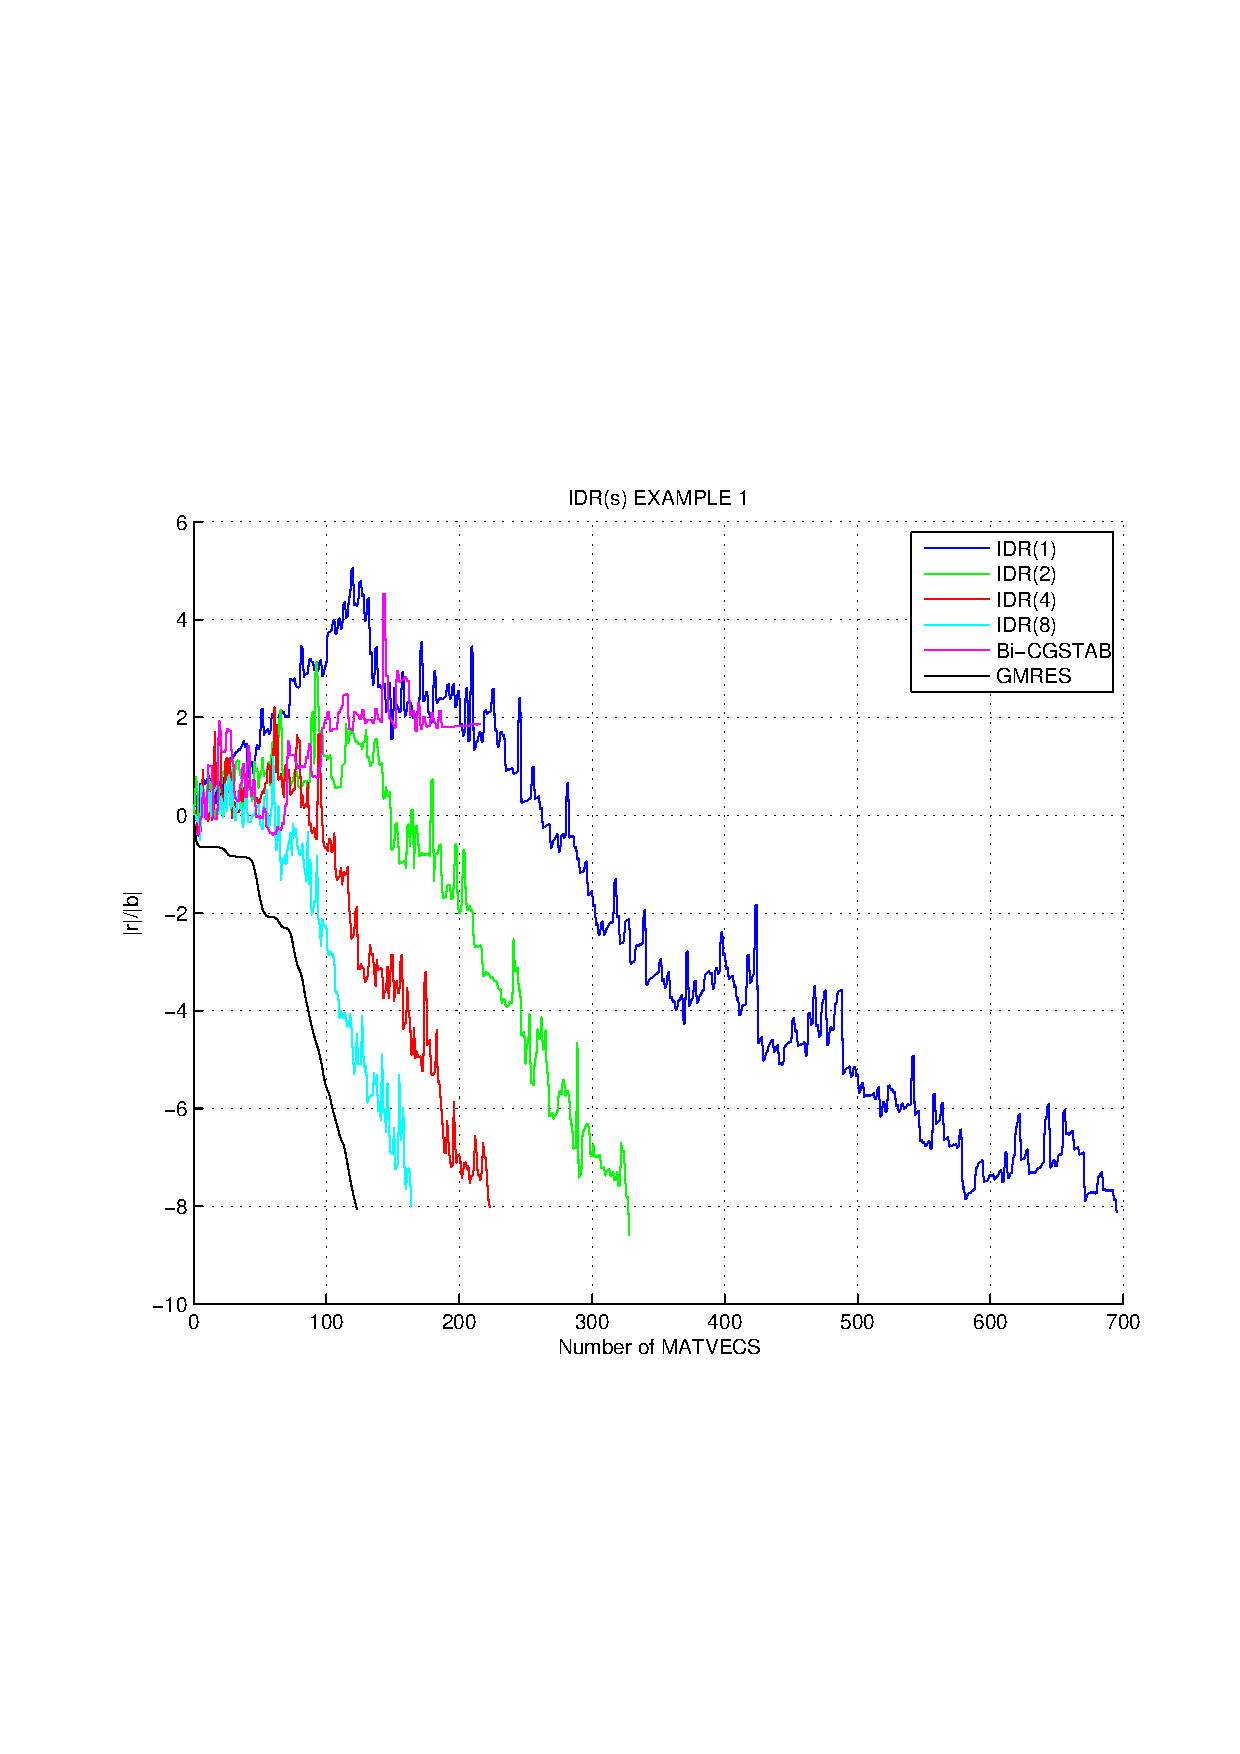
\includegraphics[width=.60\linewidth]{example1}
\caption{Convergence of unpreconditioned IDR($s$).}
\label{fig:example1}
\end{figure}
All methods achieve the required accuracy, meaning that {\tt flag = 0} and that {\tt relres < tol}, with 
{\tt tol = 1e-8} (default). Figure \ref{fig:example1} also shows the convergence of GMRES and Bi-CGSTAB. The convergence
curves of IDR($s$) are in between the convergence curves of GMRES and Bi-CGSTAB, and are increasingly closer to
the GMRES curve for higher $s$.

\subsection{Example 2: IDR($s$) with SSOR-preconditioning  using Eisenstat's trick.}
The second example shows IDR($s$) with SSOR-preconditioning. The matrix-vector multiplication and 
the preconditioning operation are combined using Eisenstat's trick.

Let 
\[
   A = L + D + U\nonumber
\]
where $L$, $D$, and $U$ are the strictly lower triangular part, the main diagonal, and the strictly upper triangular of $A$, respectively. 
The SSOR preconditioner (more accurately Symmetric Gauss-Seidel preconditioner) is defined by
\[
  B = (L+D) D^{-1} (U + D) = (L D^{-1} +I)(U + D) ~.
\]
The (two sided) preconditioned system now reads
\begin{eqnarray}\nonumber
  D (L+D)^{-1} A (U + D)^{-1} y &=&  D (L+D)^{-1}b ~,\\
  x &=& (U + D)^{-1} y
\end{eqnarray}
In order to make multiplications with the preconditioned system matrix $\tilde{A}$ more
efficient we rewrite this matrix as follows
\begin{eqnarray}\nonumber
  \tilde{A} &=& D (L+D)^{-1} A (U+D)^{-1}\\ \nonumber
            &=& D (L+D)^{-1} (L+D -D +U+D) (U+D)^{-1}\\  \nonumber
            &=& D ((U+D)^{-1} + (L+D)^{-1} - (L+D)^{-1}D(U+D)^{-1} )\\ \nonumber 
            &=& D(U+D)^{-1} + (LD^{-1}+I)^{-1} - (LD^{-1}+I)^{-1}D(U+D)^{-1}\\ \nonumber 
            &=& (UD^{-1}+I)^{-1} + (LD^{-1}+I)^{-1}(I - (UD^{-1}+I)^{-1} ) \nonumber ~.
\end{eqnarray}
The multiplication $v = \tilde{A}u$ can then be efficiently performed as follows
\begin{eqnarray}\nonumber
   t &=& (UD^{-1}+I)^{-1}u\\ \nonumber
   v &=& t + (LD^{-1}+I)^{-1}( u - t ) \nonumber ~~.
\end{eqnarray}
The above technique can be implemented as follows:
\begin{verbatim}
K.name = 'mv'; % name of the function that performs the matrix-vector multiplication
K.D = diag(diag(A)); % field K.D contains D
K.L = tril(A)/K.D; % field K.L contains (LD^{-1}+I)
K.U = triu(A)/K.D; % field K.U contains (UD^{-1}+I)
f = K.L\b; % right-hand side of preconditioned system
[y, flag,relres,iter,resvec] = idrs( K, f ); % Note: the default s=4 is taken here
x = KD\(K.U\y); % scale back
\end{verbatim}
The function {\tt mv} that performs the preconditioned matrix-vector  multiplication is as follows
\begin{verbatim}
function v = mv( u, A );
t = (A.U\u);
v = t + (A.L\( u - t ));
return
\end{verbatim}
   
Figure \ref{fig:example2} shows the convergence for IDR($s$), with $s$ = 1,2,4 and 8.
\begin{figure}
\centering
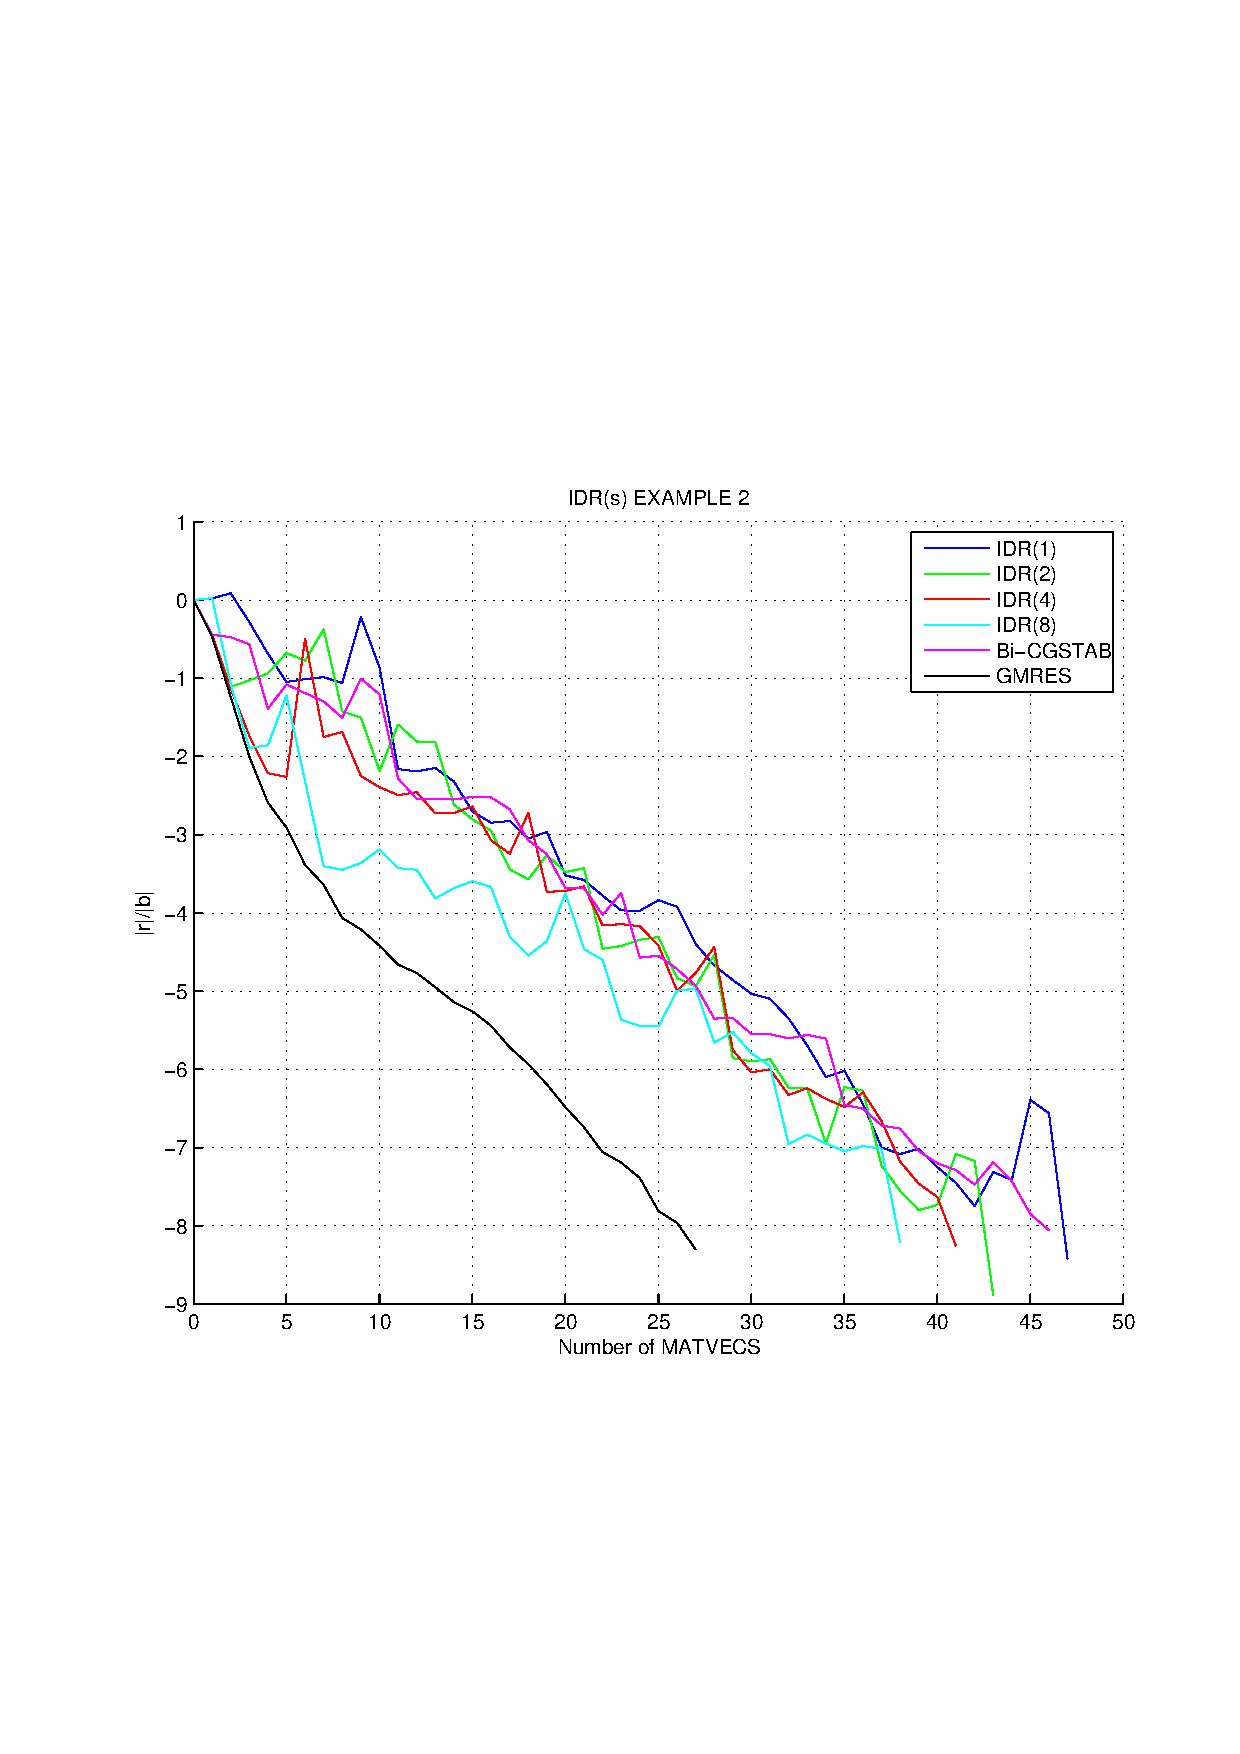
\includegraphics[width=.60\linewidth]{example2}
\caption{Convergence of IDR($s$) with SSOR preconditioner, using Eissenstat's trick.}
\label{fig:example2}
\end{figure}
As in the previous example, also the convergence curves of GMRES and Bi-CGSTAB are shown. Note that for this example
IDR($s$) does not give a significant gain over Bi-CGSTAB. The reason is that the convergence
of Bi-CGSTAB is rather close to the optimal convergence of GMRES: there is not much room for much improvement. This is
typical for well-conditioned (and well-preconditioned) problems.

For this example all methods terminate with {\tt flag = 0}, which indicates that the required accuracy is achieved.
Also, the parameter {\tt relres} is always smaller than $10^{-8}$, the default tolerance. However, if we check the
scaled residual norm $\|b - Ax\|/\|b\|$ we get a value that is much higher than the required tolerance. For example,
\begin{verbatim}
IDR(4) iteration
Relative unpreconditioned residual norm: 9.0194e-05 
|b - Ax|/|b| = 5.5186e-09
\end{verbatim}
The reason for this is that {\tt relres} ($= \|b - Ax\|/\|b\|$) corresponds to the relative residual norm for
the \emph{preconditioned} system, which may differ considerably from the relative residual norm for the
unpreconditioned system if left or two-sided preconditioning is used. The next examples use implicit preconditioning, 
which is in IDR($s$) equivalent with right-preconditioning. In this case the residual of the preconditioned system 
and of the unpreconditioned system are the same.
\subsection{Example 3: SSOR-preconditioned IDR($s$), preconditioner passed as a factored matrix}
Example 3 shows how IDR($s$) can be combined with implicit SSOR-preconditioning (in IDR($s$) this
is equivalent with right preconditioning). So in this case the preconditioned system reads
\begin{eqnarray}\nonumber
  A ((LD^{-1}+I)(U + D))^{-1} y &=&  b ~,\\
  x &=& ((LD^{-1}+I)(U + D))^{-1} y
\end{eqnarray}
The implementation in MATLAB is as follows:
\begin{verbatim}
s = 1;
tol = []; % use default
maxit = []; % use default

D = diag(diag(A));
M1 = tril(A)/D;
M2 = triu(A);

[x,flag,relres,iter,resvec] = idrs(A,b,s,tol,maxit,M1,M2);
\end{verbatim}

Figure \ref{fig:example3} shows the convergence of IDR($s$) for four choices of $s$. Again all methods terminate
with {\tt flag = 0}, meaning that the required accuracy is achieved.
\begin{figure}
\centering
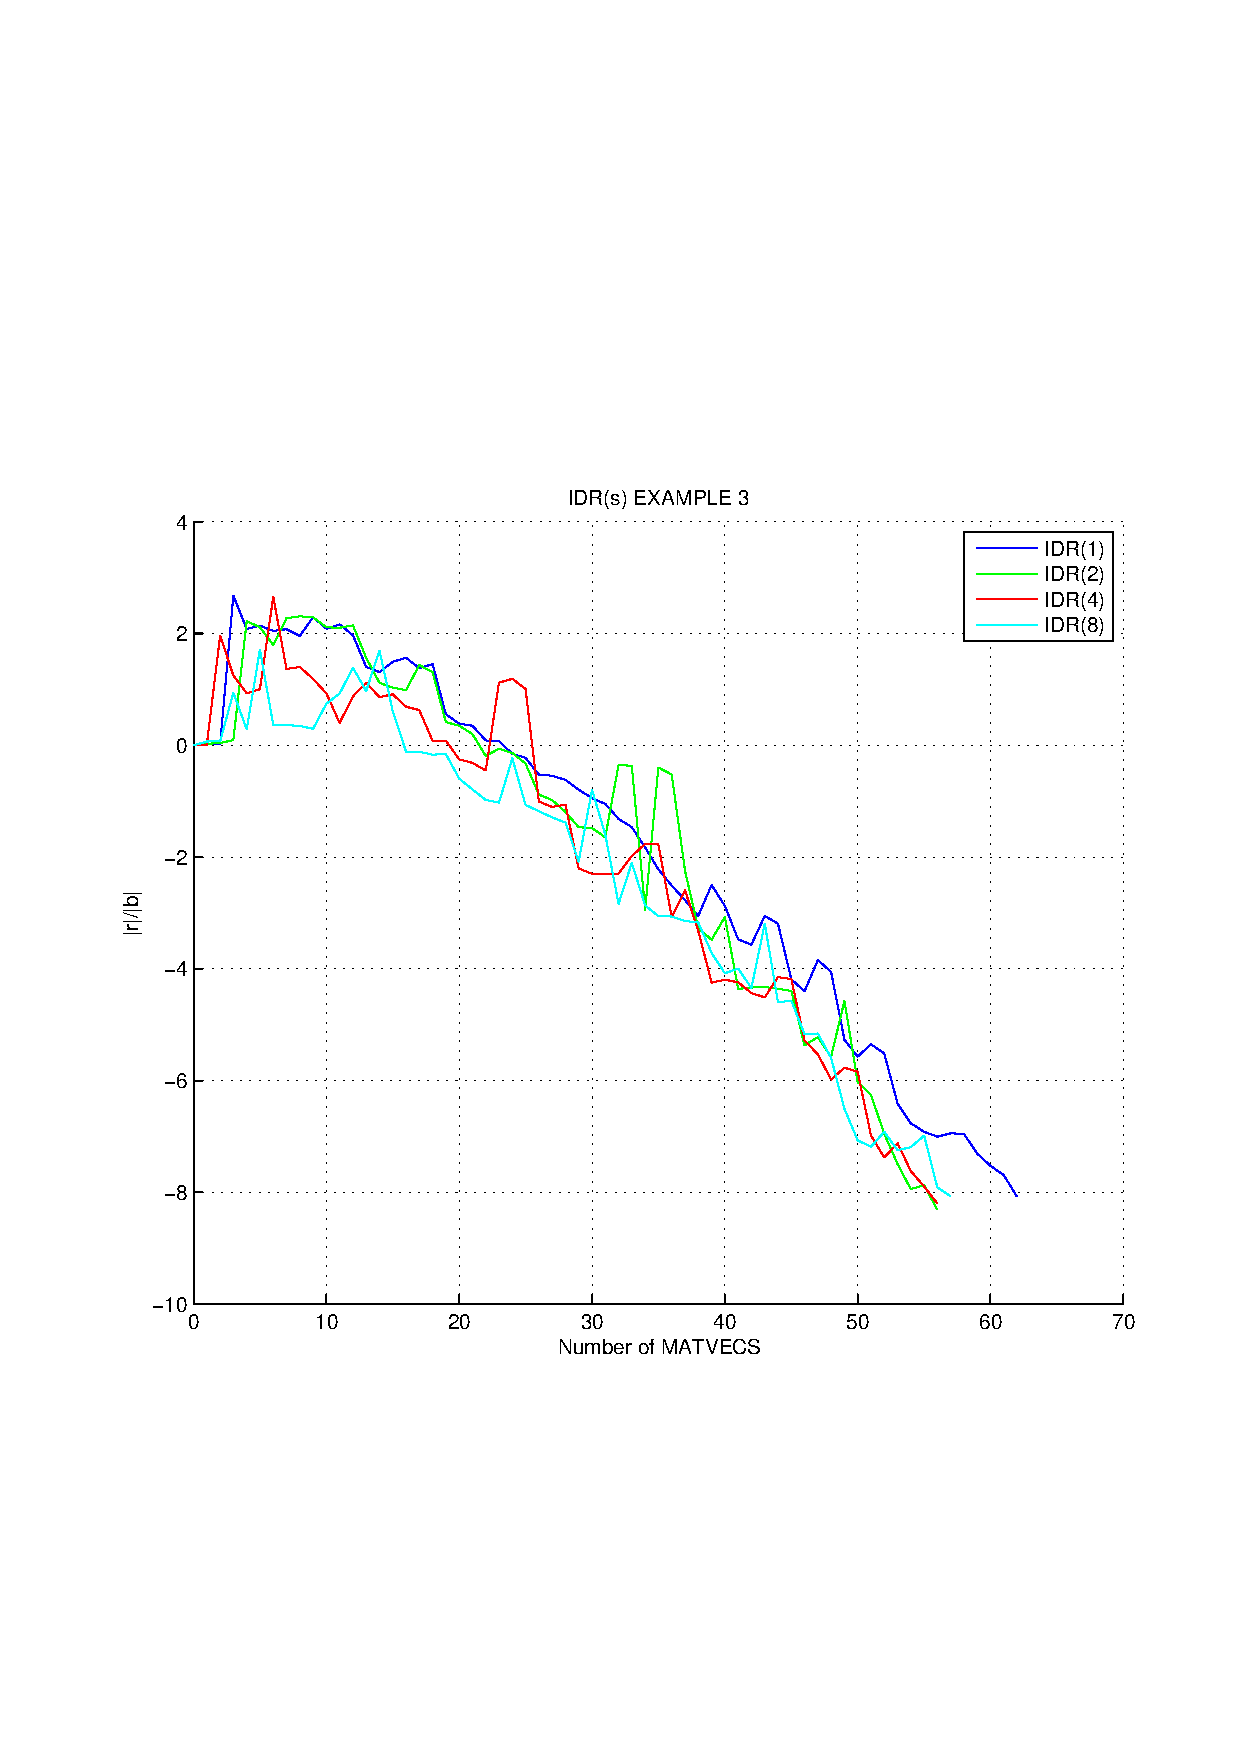
\includegraphics[width=.60\linewidth]{example3}
\caption{Convergence of IDR($s$) with SSOR preconditioning, preconditioner passed as a factored matrix.}
\label{fig:example3}
\end{figure}

\subsection{Example 4: IDR($s$) with SSOR preconditioning, preconditioner specified using functions}
Example 4 shows how the action of a  preconditioner can be passed as a function. We illustrate this with the
same preconditioner as in the previous example, where the matrix was passed via the parameter list in the form of 
a factored matrix.

The preconditioner can be passed in the form of functions that define the action of the preconditioner as follows.
\begin{verbatim}
s = 4; maxit = []; tol = [];
M1.name = 'm1';
M1.D = diag(diag(A));
M1.L = tril(A)/M1.D;
M2.name = 'm2';
M2.U = triu(A);
[x,flag,relres,iter,resvec] = idrs(A,b,s,tol,maxit,M1,M2);
\end{verbatim}
The function {\tt m1} and {\tt m2} are defined by
\begin{verbatim}
function x = m1( y, M1 );
x = M1.L\ y;
return
function x = m2( y, M2 );
x = M2.U\ y;
return
\end{verbatim}
The resulting convergence for the four different choices of $s$ is displayed in figure \ref{fig:example4}. The 
convergence curves are the same as in figure \ref{fig:example3}.
\begin{figure}
\centering
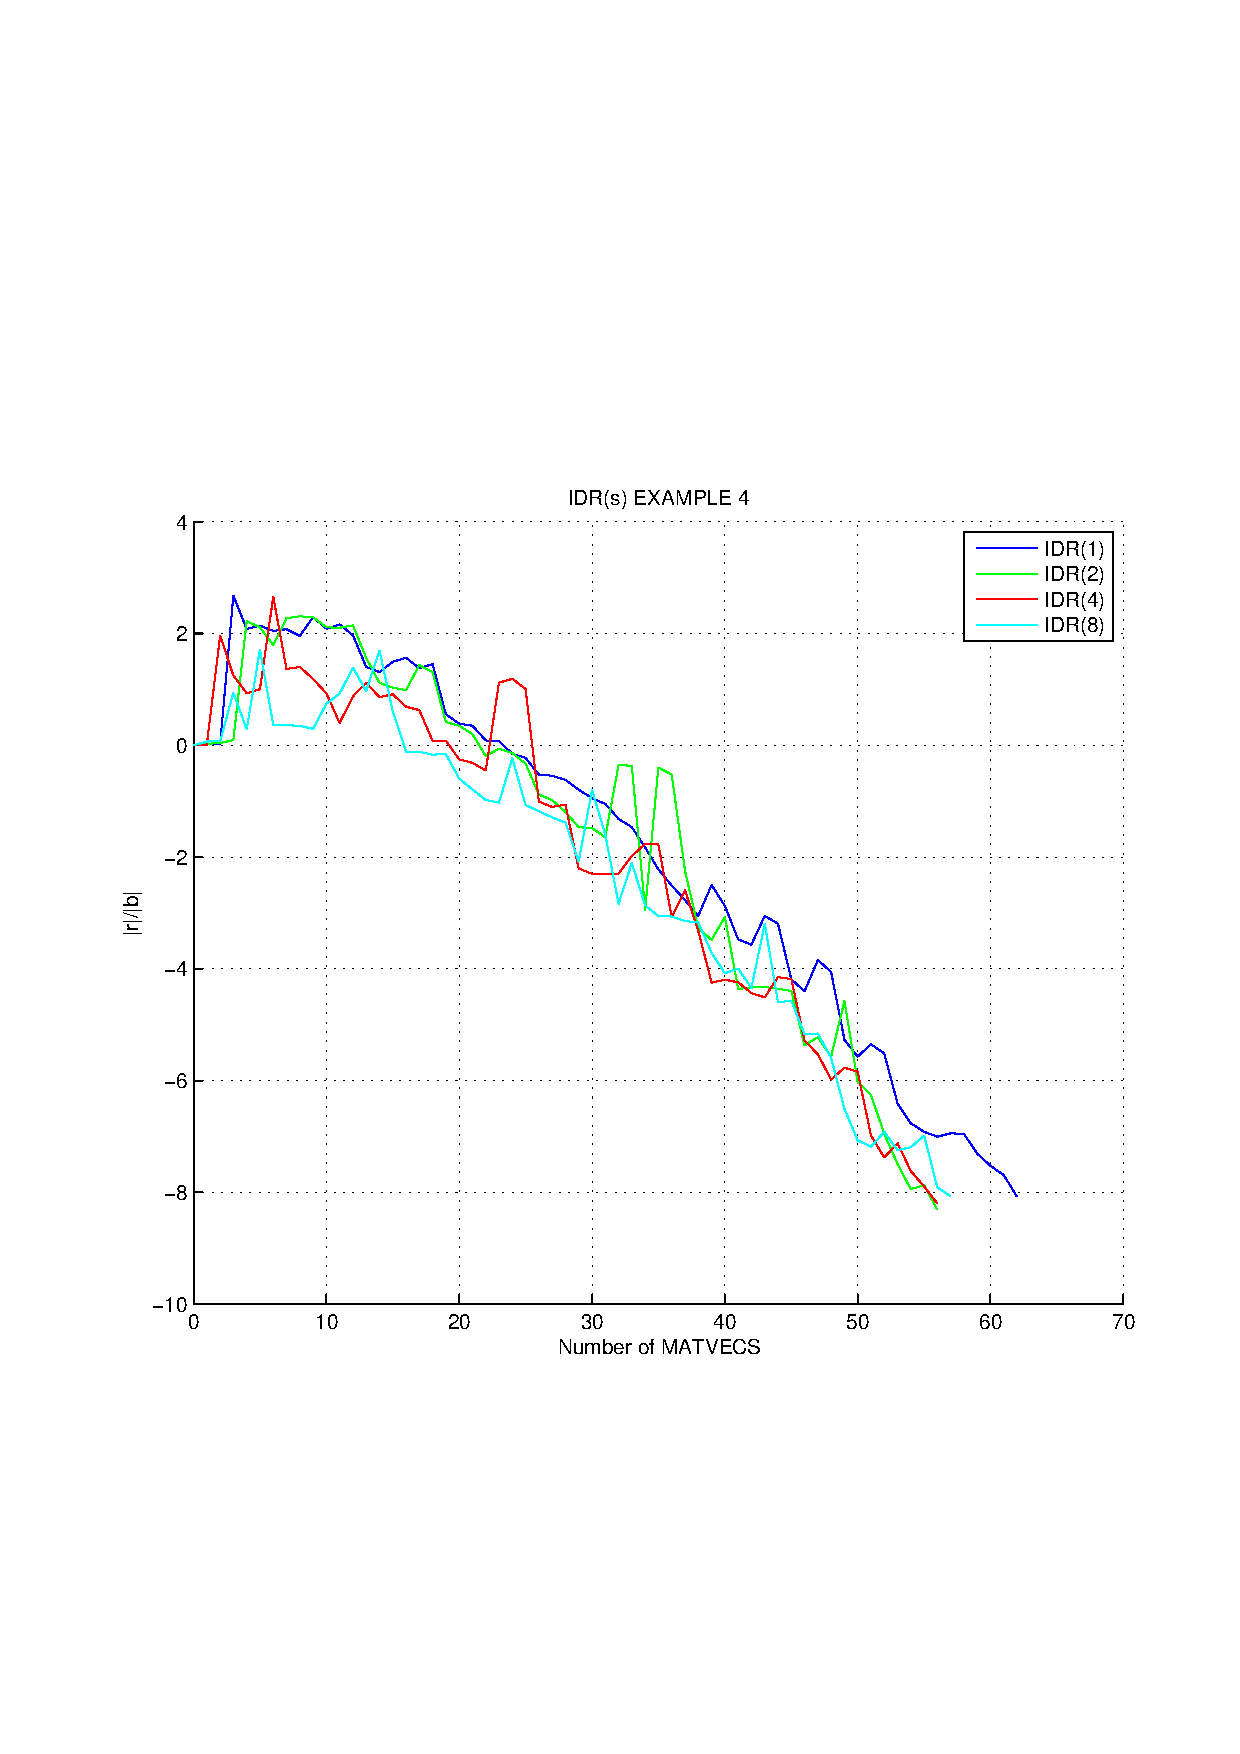
\includegraphics[width=.60\linewidth]{example4}
\caption{Convergence of IDR($s$) with SSOR preconditioning, preconditioner specified using functions.}
\label{fig:example4}
\end{figure}
\subsection{Example 5: IDR($s$) with residual smoothing}
Example 5 shows the effect of residual smoothing.

The residual norms in IDR($s$) do not decrease monotonically. However, alternative residuals with monotonically 
decreasing norms can be obtained by combining IDR($s$) with a residual smoothing algorithm. In IDR($s$) 
so-called Sch\"onauer-Weiss smoothing \cite{smoothing,weiss} is implemented. In this smoothing algorithm, 
a linear combination of the smoothed residual $\tilde{r}_{n-1}$ and the unsmoothed IDR($s$)-residual is  made in 
every iteration:
\[
   \tilde{r}_n = \tilde{r}_{n-1} - \sigma_n (\tilde{r}_{n-1} - r_n) ~~~~ \tilde{r}_0 = r_0.
\]
The parameter $\sigma_n$ is determined such that the norm of the smoothed residual is minimised, which leads to
\[
   \sigma_n = \frac{(\tilde{r}_{n-1} - r_n)^H \tilde{r}_{n-1}}{(\tilde{r}_{n-1} - r_n)^H (\tilde{r}_{n-1} - r_n)}
\]
The approximate solution vector is updated consistently with the smoothed residual as follows
\[
    \tilde{x}_n = \tilde{x}_{n-1} - \sigma_n (\tilde{x}_{n-1} - x_n) ~~~~ \tilde{x}_0 = x_0.
\]

Residual smoothing can be switched on as follows:
\begin{verbatim}
% Other parameters (defaults):
maxit = []; tol = []; M1 = []; M2 = []; x0 = [];
s = 4;
% Switch on residual smoothing:
options.smoothing = 1;
% Call idrs:
[x,flag,relres,iter,resvec] = idrs(A,b,s,tol,maxit,M1,M2,x0,options);
\end{verbatim}

Figure \ref{fig:example5} shows the convergence of IDR($s$) with smoothed residuals. This figure should be
compared with figure \ref{fig:example1} which shows the convergence of IDR($s$) without residual smoothing.
We remark that, although the smoothed residuals curves look nicer, the rate of convergence is essentially the same.
\begin{figure}
\centering
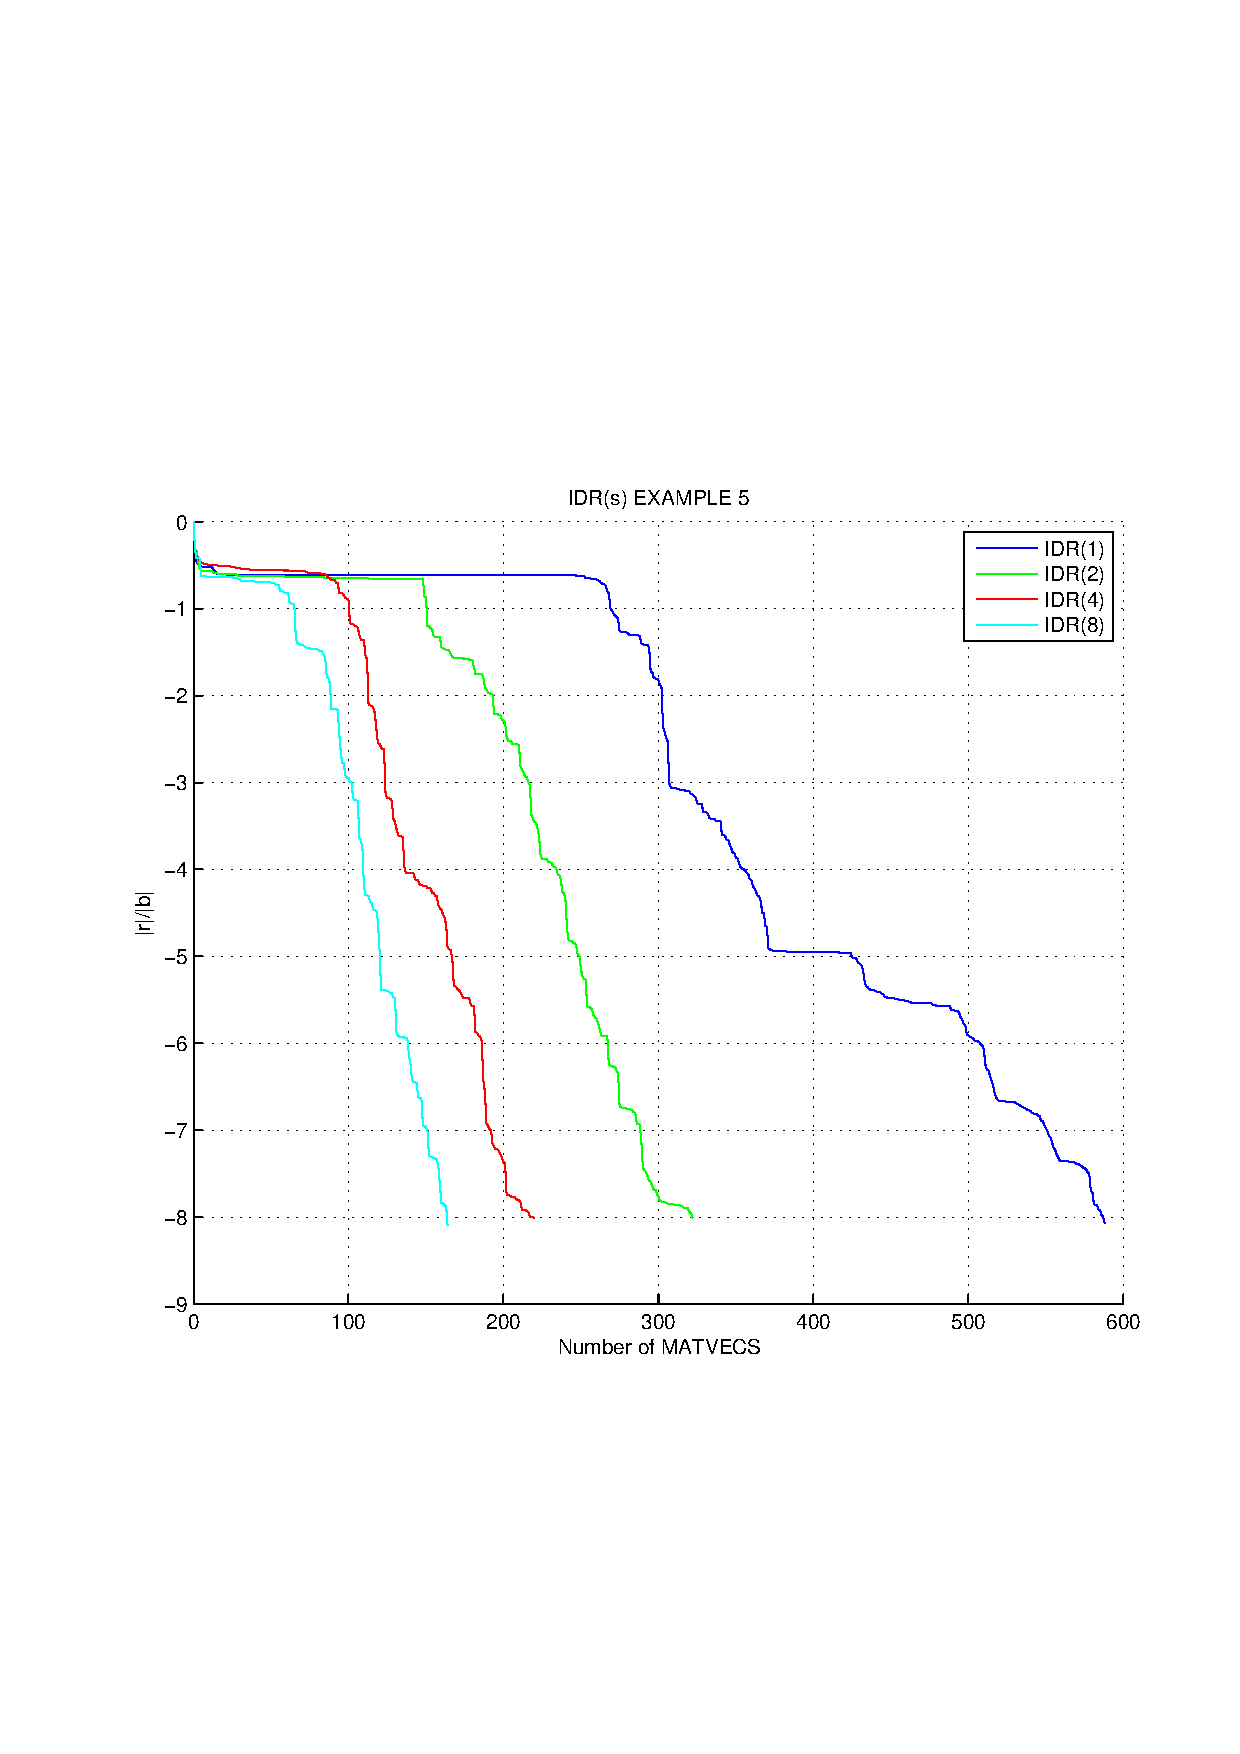
\includegraphics[width=.60\linewidth]{example5}
\caption{Convergence of IDR($s$) with residual smoothing.}
\label{fig:example5}
\end{figure}

\subsection{Example 6: IDR($s$) with a minimum residual choice for $\omega$}
Example 6 illustrates what happens if the parameter $\omega$ is chosen to minimize the residual norm. Note that
this is the standard strategy in Bi-CGSTAB. In IDR($s$), the minimum residual strategy for computing $\omega$ 
is used if {\tt idrs} is called as follows:
\begin{verbatim}
% Other parameters (defaults):
maxit = []; tol = []; M1 = []; M2 = []; x0 = [];
s = 4;
% Minimal residual choice for omega:
options.omega = 0;
% Call idrs:
[x,flag,relres,iter,resvec] = idrs(A,b,s,tol,maxit,M1,M2,x0,options);
\end{verbatim}

Figure \ref{fig:example6} shows the convergence of IDR($s$) if the minimal residual strategy for $\omega$ is used.
This figure should be compared with figure \ref{fig:example1} where the same computation is performed with the
"maintaining the convergence" strategy for $\omega$ \cite{maintaining,idrs_biortho}. The 
"maintaining the convergence" strategy corresponds with the default value {\tt options.omega = 0.7}.
\begin{figure}
\centering
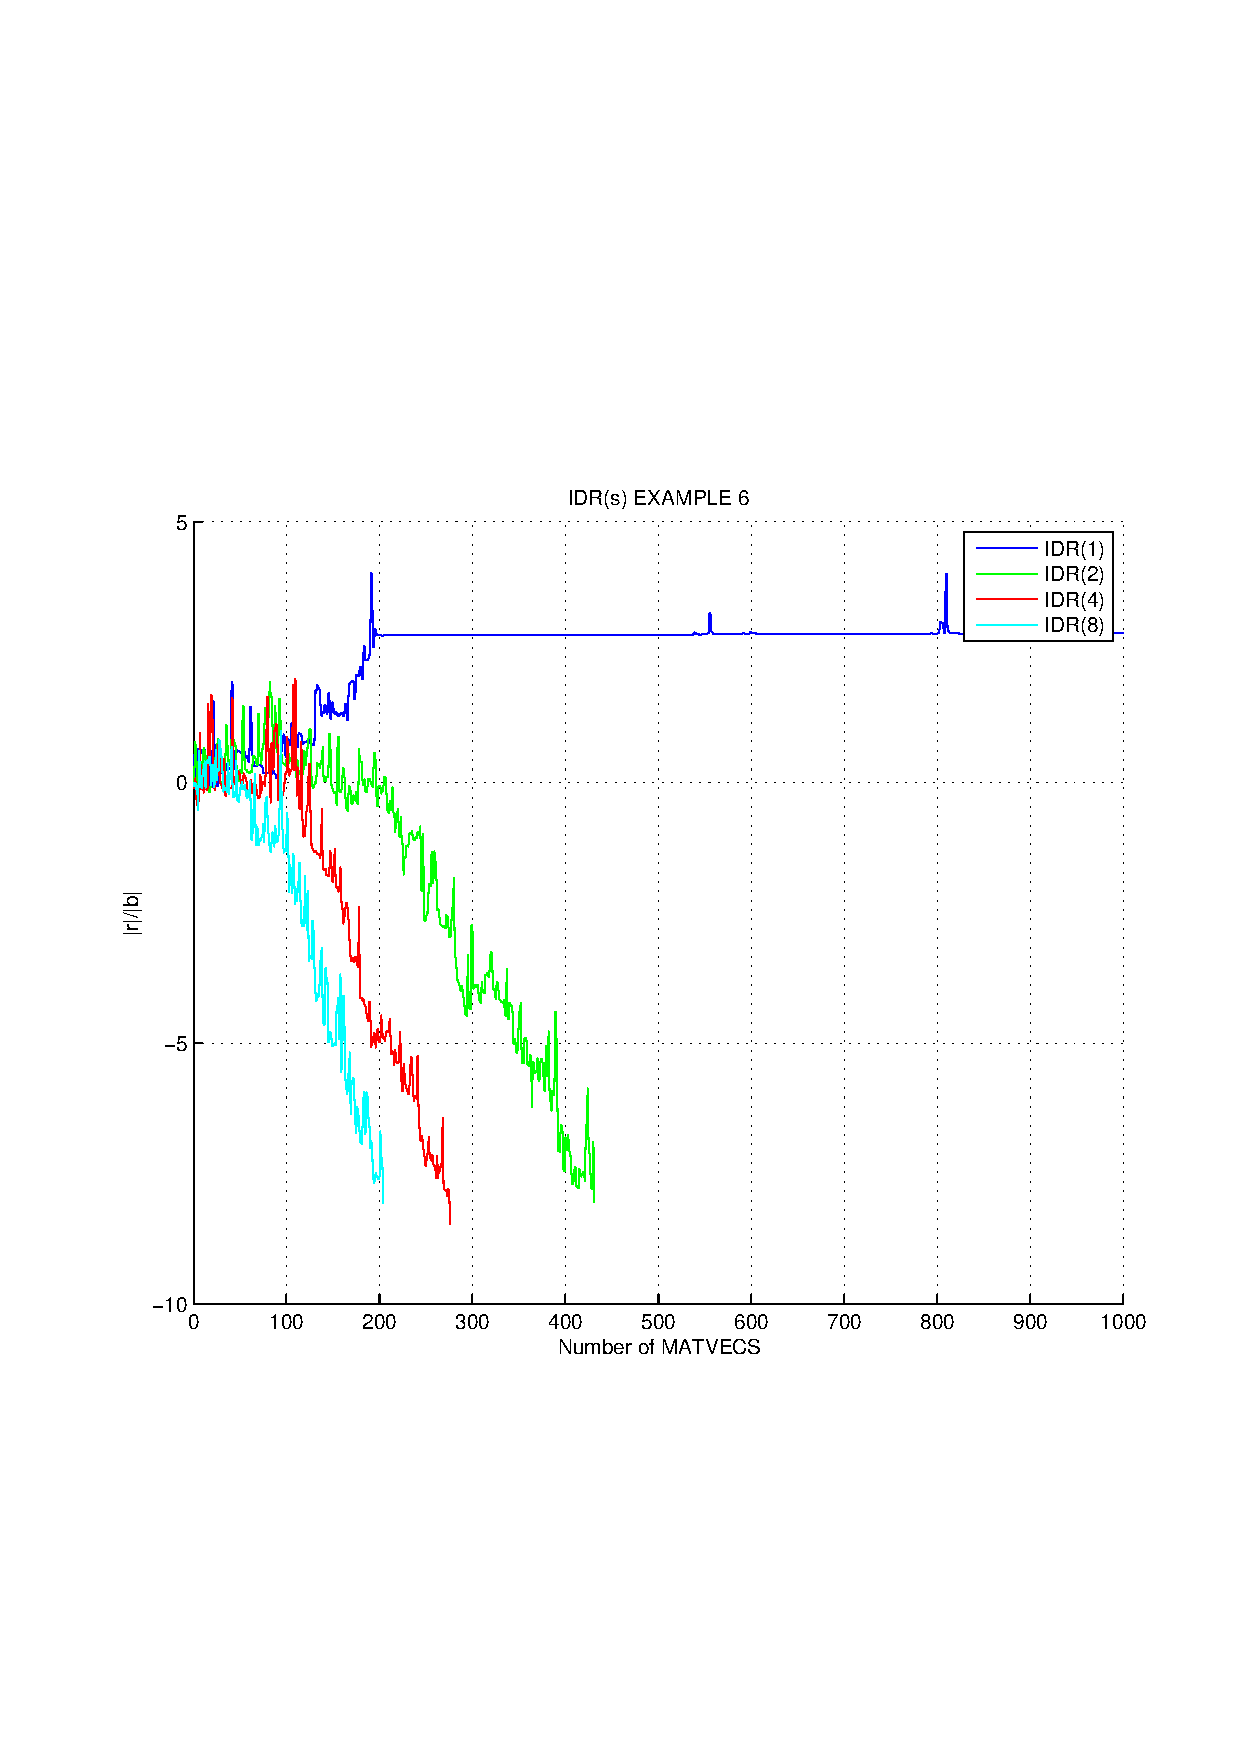
\includegraphics[width=.60\linewidth]{example6}
\caption{Convergence of IDR($s$) with minimal residual choice for $\omega$.}
\label{fig:example6}
\end{figure}
The convergence for small values of $s$ is much worse for the "minimum residual" strategy. We have this behaviour 
consistently for problems that have eigenvalues on both sides of the imaginary axis. Note that IDR(1) does
not converge within the maximum number of iterations. This results in {\tt flag = 1}.

\subsection{Example 7: IDR($s$) with complex shadow vectors}
Example 7 shows a different choice of the shadow vectors.

If $A$ is real and strongly nonsymmetric, \emph{complex} random shadow vectors may give a much faster convergence 
than \emph{real} random shadow vectors. This effect is strongest for small values of $s$. 

Complex shadow vectors can be defined and passed to {\tt idrs} as follows:
\begin{verbatim}
s = 2; tol = 1e-8; maxit = 1000;
M1 = []; M2 = []; x0 = []; im = sqrt(-1);
randn('state', 0); P = randn(n,s) + im * randn(n,s); P = orth(P); options.P = P;
[x,flag,relres,iter,resvec] = idrs(A,b,s,tol,maxit,M1,M2,x0,options);
\end{verbatim}

The resulting convergence curves for the four choices for $s$ are shown in Figure \ref{fig:example7}.
\begin{figure}
\centering
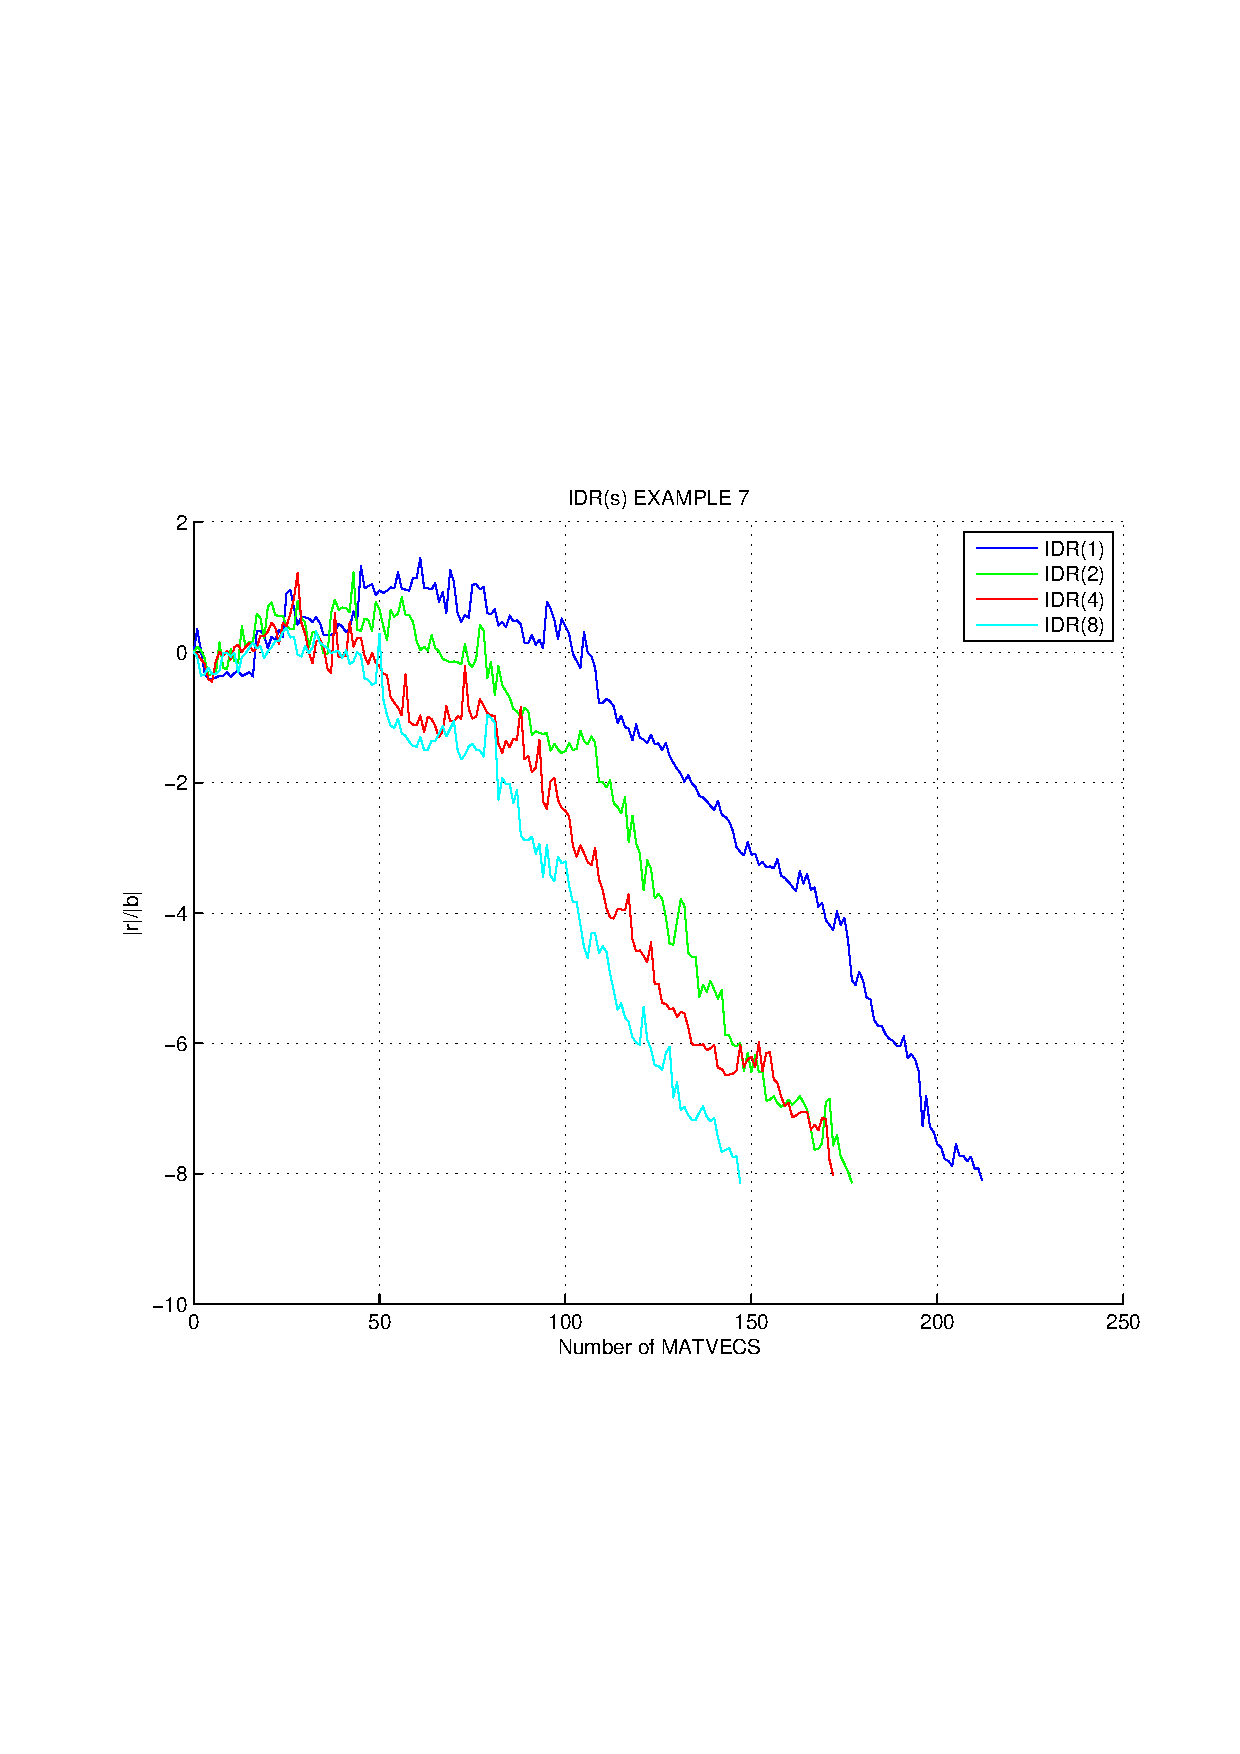
\includegraphics[width=.60\linewidth]{example7}
\caption{Convergence of IDR($s$) with complex shadow vectors.}
\label{fig:example7}
\end{figure}
Comparing Figure \ref{fig:example1} and \ref{fig:example7} shows that the complex choice for the shadow vectors gives considerably faster 
convergence for this example. The computations, however, have to be performed using
complex arithmetic, which is more expensive than real arithmetic.

\subsection{Example 8: IDR($s$) with strict tolerance}
Example 8 tries to compute the solution with a tolerance that is close to relative machine precision.

It is well known that high peaks in the initial phase of the iterative process may destroy the final achievable accuracy
if the residuals are computed recursively \cite{peaks}. An intuitive explanation of this is as follows.  In every 
iterative step \emph{relative} errors in the order of the machine precision $\epsilon$ are made. 
If the residuals are computed recursively, the errors from an
earlier stage of the process propagate through all succeeding iterations and also pollute the later residuals. 
If a residual in an early stage is very large in norm, the roundoff errors made in this phase  
can therefore cause a large relative error in the final residuals that are small in norm. 
This usually manifests itself in a large difference between the recursively updated residual $r_i$ and the true
residual $b-Ax_i$. This so-called residual gap can be so large that the final true residual is above the required 
tolerance, although the recursively computed residual is below. To illustrate this we take a strict tolerance  
$10^{-12}$, i.e., the iterative process is terminated if $\|r_i\|/\|b\| < 10^{-12}$. 
 
A sample call with $s=2$ is 
\begin{verbatim}
s = 2; tol = 1e-12;
[x,flag,relres] = idrs(A,b,s,tol);
\end{verbatim}

The resulting convergence curves for the four choices for $s$ are shown in Figure \ref{fig:example8}.
\begin{figure}
\centering
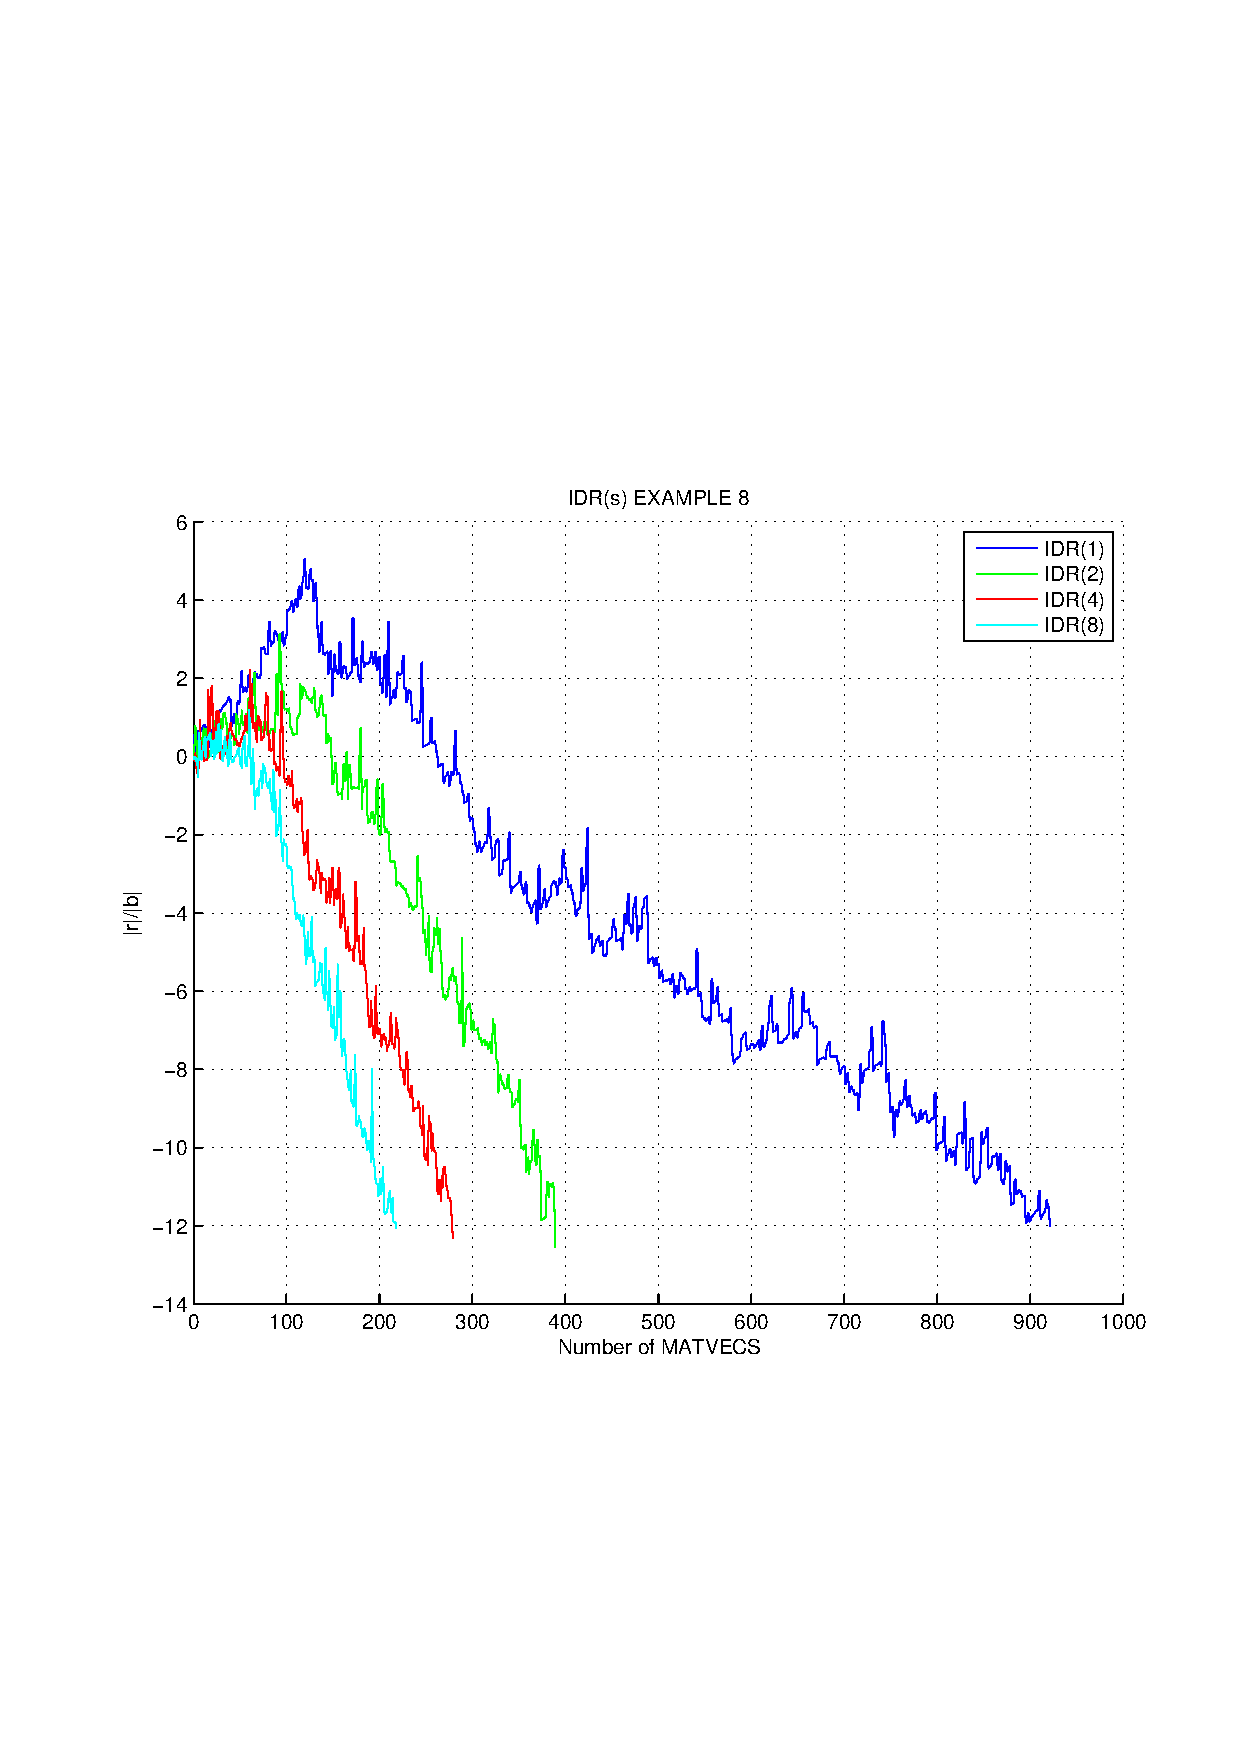
\includegraphics[width=.60\linewidth]{example8}
\caption{Convergence of IDR($s$) with strict tolerance.}
\label{fig:example8}
\end{figure}
Although the convergence curves look normal, and the norms of the recursively updated residuals divided by the norm 
of $b$ drop below the required tolerance, the relative norms of the true final residuals are all above the tolerance. 
For example, for IDR(1) we get {\tt flag = 2}, which indicates that the true relative residual norm is above the 
tolerance, and {\tt relres = 2.7328e-11}. Note, {\tt relres} is equal to the norm of the final residual
divided by the norm of $b$, and should be smaller than {\tt tol}. 

In the next two examples we will show two possible solutions to this problem. 

\subsection{Example 9: IDR($s$) with residual replacements}
Example 9 shows the effect of a few replacements of the recursively computed residual by the true residual.

A possible cure to the loss of accuracy due to high peaks in the initial phase of the iterative process is to replace 
the recursively computed residual by the true residual once the residual norm has decreased to a sufficiently lower 
level after the peak. This moment has to be chosen carefully, since replacement of small residuals may negatively  
affect the rate of convergence, and the replacement of a residual that is too large in norm 
(to close to the peak value) may not result in a more accurate solution. Moreover, a residual replacement
requires an extra matrix-vector multiplication. The number of residual replacements should therefore be limited  for 
efficiency reasons.
We refer to \cite{reliable} for a detailed analysis and an advanced residual replacement strategy. 
 
In {\tt idrs} the following simple replacement strategy is implemented: \\
A peak is considered dangerously high if 
\[  
   \| r_i \| / \|b\| > C( {\tt tol}/ \epsilon ) ~.
\]
with $\epsilon$ the relative machine precision. The factor ${\tt tol}/ \epsilon$ corresponds to the size of a 
finite precision number that is so large that the absolute round-off error in this number,
when propagated through the process, makes it impossible to achieve the required accuracy.
The factor $C$ accounts for the accumulation of round-off errors.  This parameter has been set to $10^{-3}$.
If such a dangerous peak has been encountered, the recursively computed residual is replaced by the true residual 
once the relative norm of the residual drops below 1 (i.e., when the residual is smaller in norm than $b$).
We remark that the above residual replacement strategy improves the accuracy if high peaks occur, but it does not guarantee that the final true 
residual is below the required tolerance.

A sample call with $s=4$ is 
\begin{verbatim}
s = 4; tol = 1e-12; maxit = [];
M1 = []; M2 = []; x0 = [];
options.replace = 1;
[x,flag,relres,iter,resvec,repl] = idrs(A,b,s,tol,maxit,M1,M2,x0,options);
\end{verbatim}
 
The resulting convergence curves are shown in Figure \ref{fig:example9}.
\begin{figure}
\centering
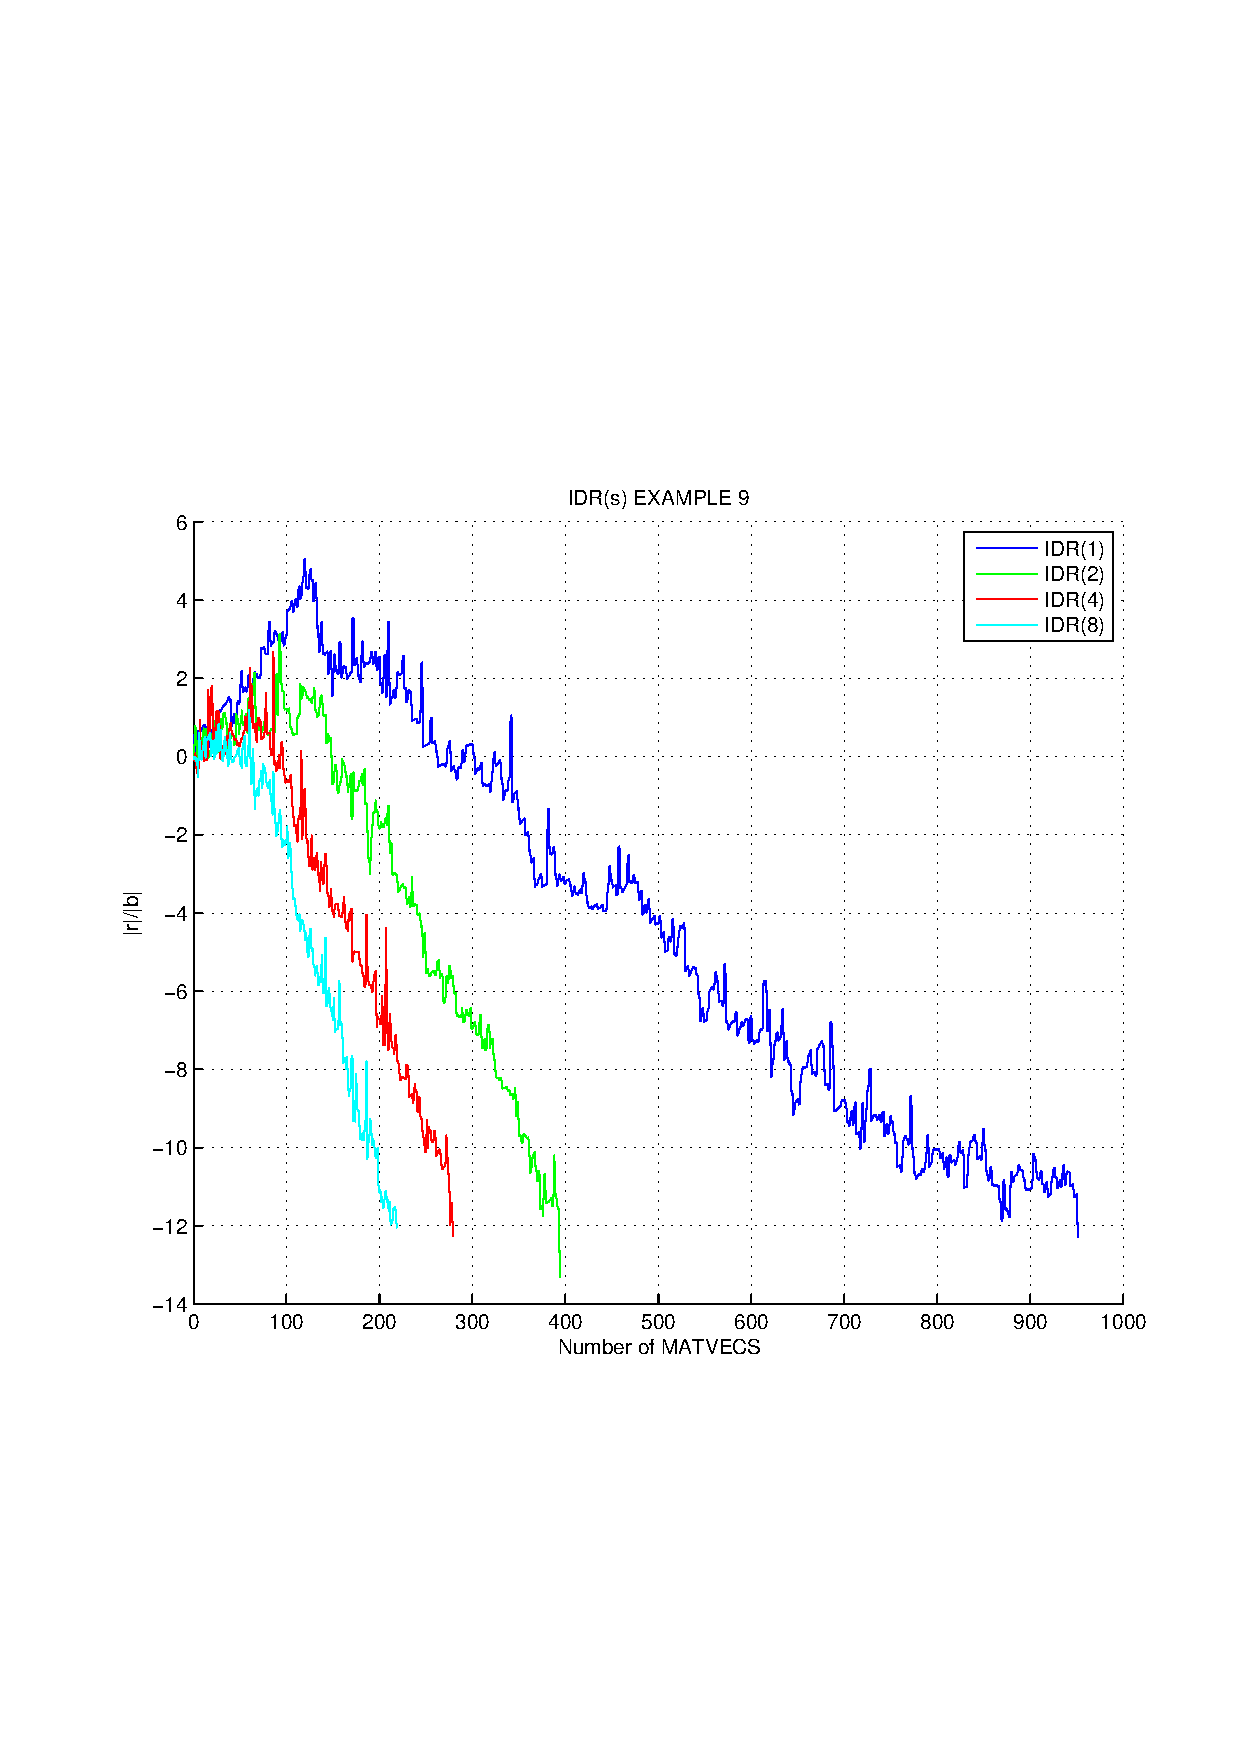
\includegraphics[width=.60\linewidth]{example9}
\caption{Convergence of IDR($s$) if a residual replacement strategy is used.}
\label{fig:example9}
\end{figure}
Note that the rate of convergence is slightly negatively affected if the residual replacement strategy is used. The accuracy of the solution,
however, has improved. For example for $s=1$ we get {\tt relres = 5.1644e-13} and {\tt flag = 0}, whereas in the previous example we had 
{\tt relres = 2.7328e-11} and {\tt flag = 2}. 

\subsection{Example 10: IDR($s$) with a restart}
Example 10 shows how to improve the final accuracy by restarting the process. 

An alternative way to improve the accuracy if the required tolerance is not met, is to restart the process with
the found solution as initial guess. A sample call with $s= 2$ to implement this is:
\begin{verbatim}
s = 2; tol = 1e-12; maxit = []; M1 = []; M2 = [];
[x,flag,relres,iter,resvec] = idrs(A,b,s,tol,maxit);
if ( flag > 0 ) [x,flag,relres,iter,resvec] = idrs(A,b,s,tol,maxit,M1,M2,x); end;
\end{verbatim}

The convergence curves are shown in Figure \ref{fig:example10}.
\begin{figure}
\centering
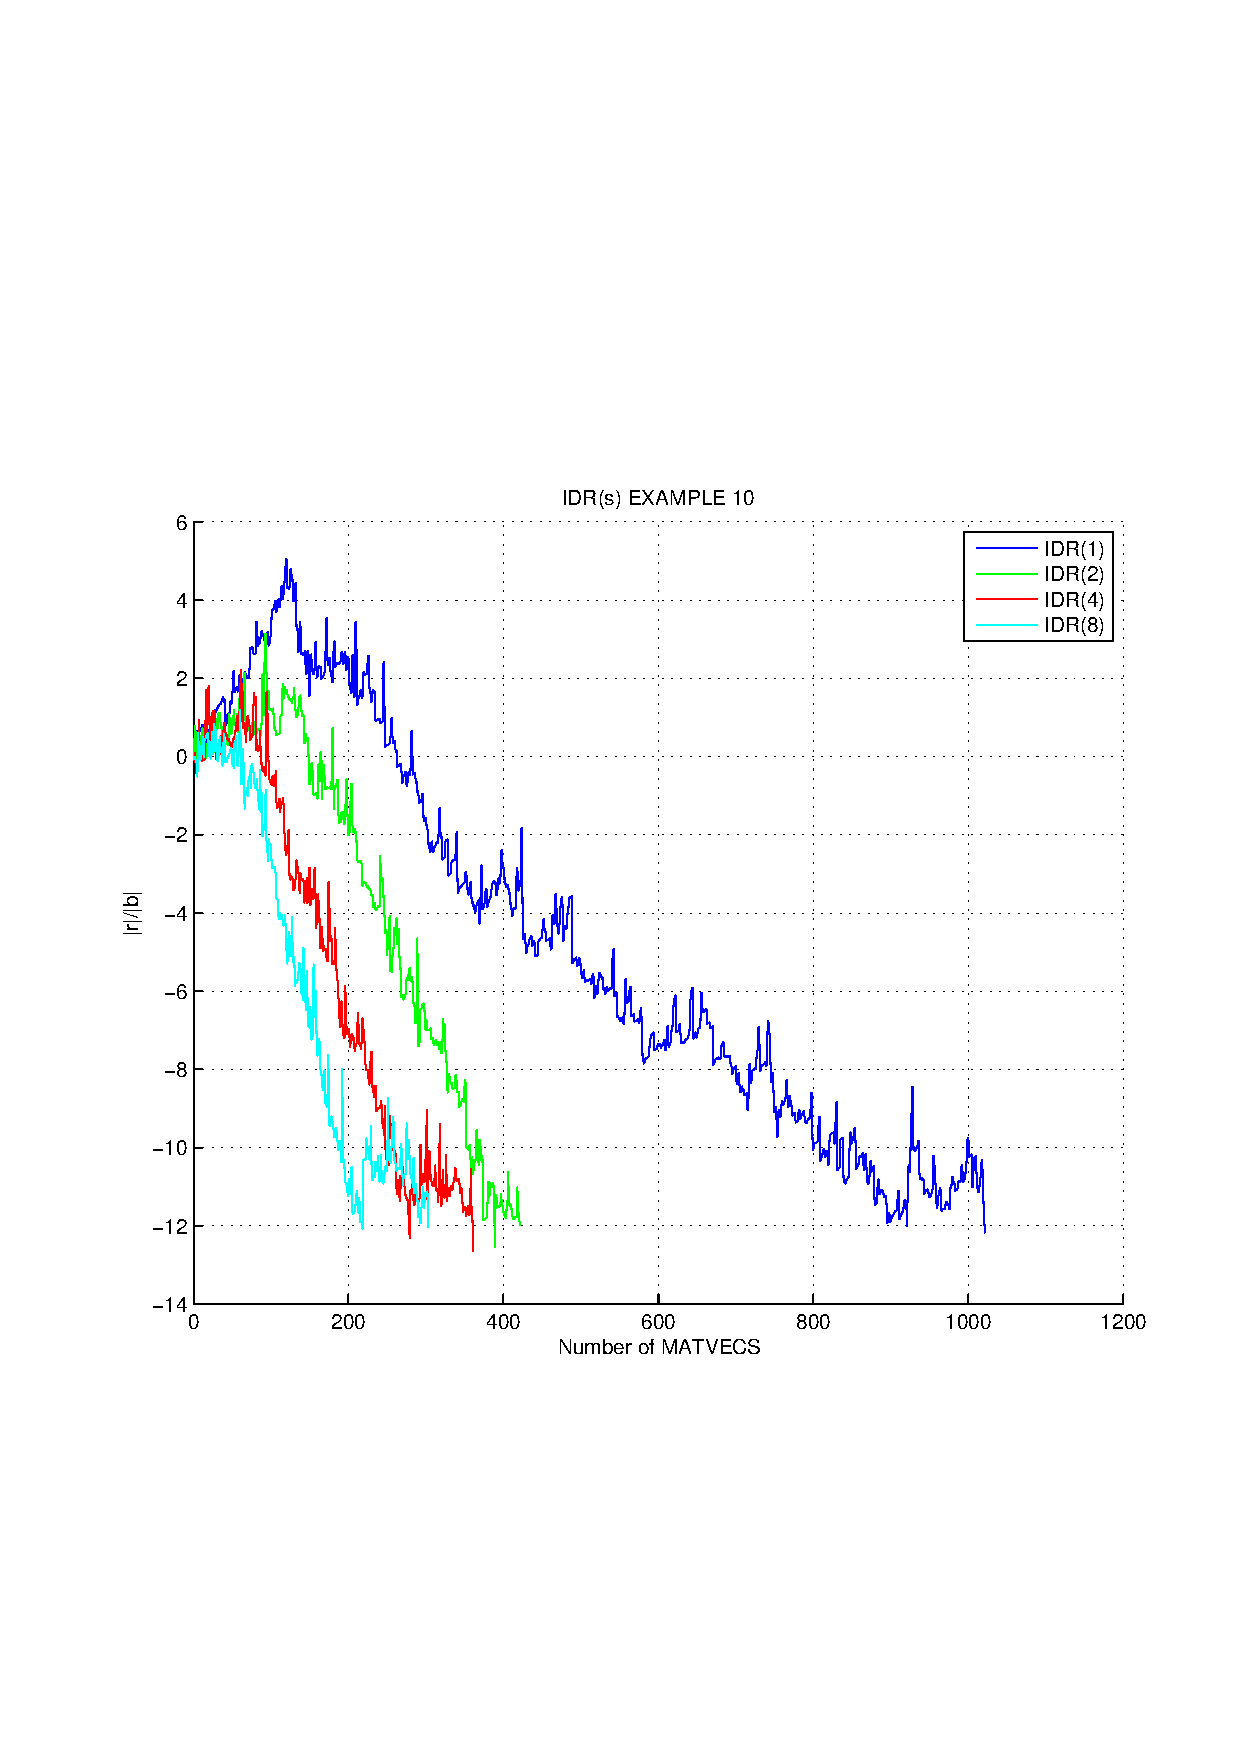
\includegraphics[width=.60\linewidth]{example10}
\caption{Convergence of IDR($s$) with a restart.}
\label{fig:example10}
\end{figure}
After restart, all processes successfully terminate with {\tt flag =0} and an accuracy that is below the tolerance.

\subsection{Example 11: equivalence of IDR(1) and Bi-CGSTAB}
Example 11 shows that IDR(1) and Bi-CGSTAB are mathematically equivalent for a certain choice of parameters.

It is well known, see \cite{idrs} that Bi-CGSTAB and IDR(1) are mathematically equivalent if the shadow vector 
$p$ is chosen the same in both methods, and if $\omega$ is
computed in the same way. The classical choices for these parameters in Bi-CGSTAB are: $p = r_0$, and $\omega$ is
computing via the minimal residual strategy.

The call to make IDR(s) mathematically equivalent to Bi-CGSTAB is therefore:
\begin{verbatim}
s = 1; tol = 1e-8; maxit = 40;
M1 = []; M2 = []; x0 = [];
options.P = b; options.omega = 0;
[x,flag,relres,iter,resvec] = idrs(A,b,s,tol,maxit,M1,M2,x0,options);
\end{verbatim}
 
Figure \ref{fig:example11} shows the convergence in the first 20 iterations of Bi-CGSTAB (Bi-CGSTAB performs 2
matrix-vector multiplications per iteration)  and in the first 40 iterations of IDR(1) with the above  choice of 
parameters.
\begin{figure}
\centering
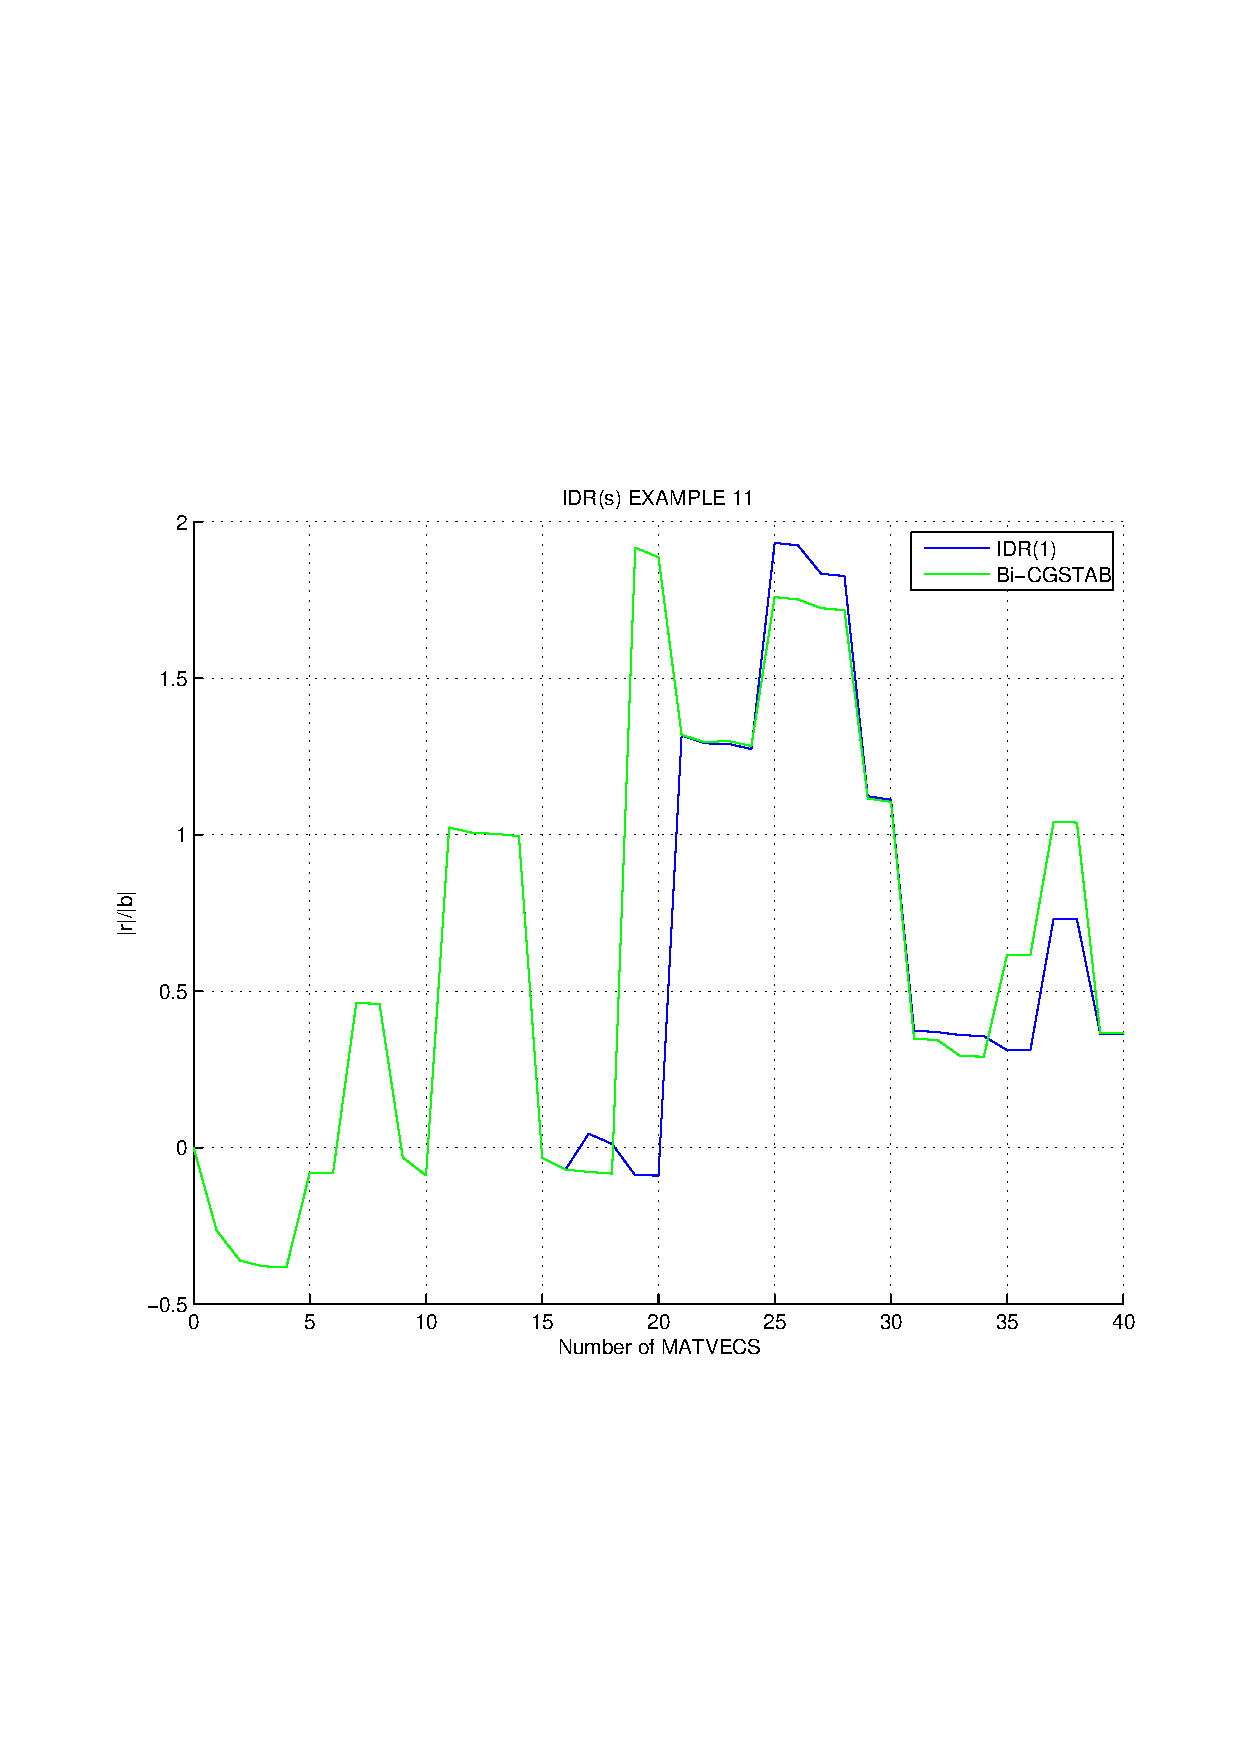
\includegraphics[width=.60\linewidth]{example11}
\caption{Equivalence of IDR(1) and Bi-CGSTAB.}
\label{fig:example11}
\end{figure}
Clearly, the convergence curves coincide until finite precision effects start to play a role. 

\begin{thebibliography}{99}

\bibitem[\protect\citeauthoryear{Greenbaum}{Greenbaum}{1997}]{peaks}
{\sc Greenbaum, A.} 1997.
Estimating the attainable accuracy of recursively computed residual methods. 
{\em SIAM J. Matrix Anal. Appl.}, 18(3):535--551.

\bibitem[\protect\citeauthoryear{Sch\"onauer}{Sch\"onauer}{1987}]{smoothing}
{\sc Sch\"onauer}, W. 1987.
{\em Scientific Computing on Vector Computers}, Elsevier, Amsterdam.

\bibitem[\protect\citeauthoryear{Sleijpen and van der Vorst}{
Sleijpen  and van der Vorst}{1995}]{maintaining}
{\sc  Sleijpen, G.L.G.} and {\sc  van der Vorst, H.A.} 1995.
Maintaining convergence properties of BiCGstab methods in finite precision arithmetic.
{\em Numerical Algorithms}, 10:203--223.

\bibitem[\protect\citeauthoryear{Sleijpen and van der Vorst}{
Sleijpen  and van der Vorst}{1996}]{reliable}
{\sc Sleijpen, G.L.G. } and {\sc van der Vorst, H.A.} 1996.
Reliable updated residuals in hybrid Bi-CG methods. {\em Computing} 6:141--163.

\bibitem[\protect\citeauthoryear{Sonneveld and van Gijzen}{
Sonneveld  and van Gijzen}{2008}]{idrs}{\sc Sonneveld, P.} 
and {\sc van Gijzen, M.B.} 2008.
IDR(s): a family of simple and fast algorithms for solving large nonsymmetric linear systems.
{\em SIAM J. Sci. Comp.}, 31(2):1035--1062.

\bibitem[\protect\citeauthoryear{van Gijzen and Sonneveld}{
van Gijzen and Sonneveld}{2011}]{idrs_biortho}
{\sc van Gijzen, M.B.} and {\sc Sonneveld, P.} 
An elegant {IDR}($s$) variant that efficiently exploits bi-orthogonality properties.
{\em ACM Transactions on Mathematical Software}, to appear.

\bibitem[\protect\citeauthoryear{Weiss}{
Weiss}{1990}]{weiss}
{\sc Weiss. R.} 1990. { Convergence Behavior of Generalized Conjugate 
Gradient Methods,} PhD thesis, University of Karlsruhe.

\end{thebibliography}

\end{document}
